\chapter{Introduction} 

\pagenumbering{arabic}
\renewcommand{\thepart}{{\Roman{part}}}	

Fishery managers have only one ``lever'' to pull when it comes to fishery management: the ability to set harvest quotas.  Fishermen work within these quotas by exerting various levels of fishing effort.  Production models have been designed to help managers and fishermen understand the ecosystem they work within and the implications of their decisions.  In this context, a production model is a mathematical model, based on data, that simulates interactions between species and predicts species biomass as a function of the distribution of fish species population, fishing effort, climate change, and other variables.  MS-PROD is a multispecies production model developed by NOAA scientists Gamble and Link \citeyearpar{gamble2009}.  A visualization may enhance such a model by making its inner workings more explicit and may be useful for decision making. The goal of this research has been to explore design alternatives and evaluate the effectiveness of different modes of portrayal and interaction to make a visualization of the MS-PROD model that will be a valuable tool to modelers and stakeholders alike. 

\section{Models}

Both the short- and long-term effects of human exploitation on an ocean ecosystem, such as the species inhabiting the Gulf of Maine, are not easily understood.  Experiments that would allow ecosystem managers to investigate the impact of different levels of exploitation over many years are either impractical or impossible to conduct on a large scale.  Fortunately, ecosystem models can be used instead to help gain a better understanding of an ecosystem.

\subsection{Lotka-Volterra Equations}

Ecosystem models are abstract representations of an ecological system, and can range from an individual species in its environment to an entire community of species.  A classic example is the Lotka-Volterra model, which is a pair of differential equations for describing the non-linear interactions between a predator species and a prey species \cite{lotka1926, volterra1926}:

\begin{align}
   \frac{d N_1}{dt} &=   N_1 \left(\alpha - \beta  N_2\right) 
\\ \frac{d N_2}{dt} &= - N_2 \left(\gamma - \delta N_1\right)
\end{align}
where $N_1$ is the number of prey animals, $N_2$ is the number of predator animals, $t$ is time, $\alpha$ is the prey animals' growth rate, $\beta$ is the rate at which the predators destroys the prey animals, $\gamma$ is the death rate of the predators, and $\delta$ is the rate at which the predators increase from consuming the prey animals.  The model can be generalized to discuss an arbitrary number of species rather than just a single pair.

The Lotka-Volterra model can be modified to take competition instead of predation into account, as in the Rosenzweig-MacArthur model \cite{rosenzweig1963} and the Leslie-Gower model \cite{leslie1960}.  These adaptations also consider carrying capacity, which is the maximum number of a species that can be sustained indefinitely in a particular environment:

\begin{align}
   \frac{d N_1}{dt} &= r_1 N_1 \left(1 - \left(\frac{N_1 + \alpha_{12} N_2}{K_1}\right)\right)
\\ \frac{d N_2}{dt} &= r_2 N_2 \left(1 - \left(\frac{N_2 + \alpha_{21} N_1}{K_2}\right)\right)
\end{align}
where $r_i$ is the growth rate for species $i$, $K_i$ is the carrying capacity for species $i$, and $\alpha_{ij}$ is the effect species $j$ has on species $i$.  As with Lotka-Volterra, this model concerns only two species, but it can be generalized to include more than two.

Both Lotka-Volterra and Leslie-Gower do not incorporate a factor that is critical when discussing fisheries management: the effect of harvest.  The Schaefer model adds a term to account for the effect of harvest on an individual species \cite{schaefer1957}:

\begin{align}
   \frac{d N}{dt} &= r N \left(1 - \left(\frac{N}{K}\right)\right) - q E N
\end{align}
where $N$ is the number (or biomass) of the species, $r$ is the growth rate, $K$ is the carrying capacity, $q$ is the catchability coefficient, and $E$ is the fishing effort.

Simple models, when available and correct, are generally preferred; since fewer components are needed to describe their real-world counterparts, they are more easily understood and implemented.  All three of these models are subjectively simple in that they only consider a few ecological factors each. However, in reality, ecosystems are complex systems that require management that recognizes them as such \cite{christensen1996}.  Thus, a more holistic approach called ecosystem-based fishery management (EBFM) has been advocated \cite{united1999}.  However, this approach has not often been implemented due to a lack of models that consider all necessary ecological factors.  Gamble and Link developed a multispecies production model (MS-PROD) to fill this gap \citeyearpar{gamble2009}.

\subsection{The MS-PROD Model}

The MS-PROD model forecasts biomass for species separated into functional groups, which are biological groupings of species that perform similar functions within their ecosystem.  The model is built upon the Schaefer production model and also includes Lotka-Volterra terms for predation, Leslie-Gower terms for competition, and carrying capacities for functional groups ($K_G$) as well as for the entire system ($K_{\sigma}$):

\begin{equation}
\frac{d N_i}{dt} = \redub{r_i}_{\substack{\text{Growth}\\\text{rate}}} N_i \left(\redub{1 - \frac{N_i}{K_G}}_{\substack{\text{Prevents}\\\text{infinite}\\\text{growth}}} - \redub{\frac{\displaystyle\sum\limits_{j=1}^g \beta_{ij} N_j}{K_G} - \frac{\displaystyle\sum\limits_{j=1}^G \beta_{ij} N_j}{K_{\sigma} - K_G}}_{\substack{\text{Competition}}} \right) - \redub{N_i \displaystyle\sum\limits_{j=1}^P \alpha_{ij} N_j}_{\substack{\text{Predation}}} - \redub{H_i N_i}_{\substack{\text{Harvest}}}
\end{equation}
where $N_i$ is the number (or biomass) of species $i$, $t$ is a unit of time, $r_i$ is growth rate for species $i$, $\beta_{ij}$ is the competition of species $j$ on $i$, $\alpha_{ij}$ is the predation of species $j$ on $i$, $H_i$ is the harvest rate on species $i$, $g$ is the number of species within species $i$'s group, $G$ is the number of groups, and $P$ is the number of predators.

This model is distinguished from other multispecies production models by describing stocks with explicit ecological and harvest factors.  Each species to be included in the simulation must be specified in the parameter file by listing growth rate, functional group membership, initial biomass, carrying capacity, and catchability.  Additionally, matrices representing inter-species relationships must be provided to describe the relationship between every pair of species.  Such matrices are required for \textit{predation}, where one species consumes the other, and \textit{competition}, where one species affects the other in any manner besides predation.  (In ecology, the word ``interaction'' is often used instead of ``competition,'' but we have chosen to use ``competition'' so that the term ``interaction'' will not be overloaded since ``interaction'' has a separate meaning in a visualization context.)

The MS-PROD authors provided us with a parameter file that contains ten key species chosen from the Northeast United States Continental Shelf Large Marine Ecosystem (NEUS LME), listed here by functional group (in bold):
\begin{itemize}
	\item \textbf{Elasmobranchs:} Skates, Spiny Dogfish
	\item \textbf{Flatfish:} Windowpane, Winter Flounder, Yellowfin Tuna
	\item \textbf{Groundfish:} Cod, Haddock, Redfish
	\item \textbf{Small Pelagics:} 	Herring, Mackerel
\end{itemize}
%Given an input parameter set of initial biomass values, a predation matrix, an interaction matrix, catchability values, and harvest effort values,
The MS-PROD model runs simulations for 30 years with an annual time step to predict individual biomasses.  While this output information is potentially valuable to fishery managers, it lacks an interactive graphical user interface.  

\section{Visualization Methods}

When designing any complex interactive visualization, a large number of design choices must be made.  This section reviews existing research of visualization methods that have relevance to the problem of creating an effective interface to a fisheries ecosystem model---in particular, methods for representing time series, networks, causality, and uncertainty.

\subsection{Time Series}

Fisheries management is focused on the sustainability of choices concerning fish stocks.  A main purpose of ecosystem management is to ensure that future generations can enjoy the same natural resources \cite{christensen1996}.  As such, the MS-PROD model provides biomass forecasts for 30 years.  Therefore, visualization techniques for temporal data must be explored.

\subsubsection{Line Charts}

\begin{figure}[h]
	\centering
	\includegraphics[width=0.9\textwidth]{figures/png/PlayfairTimeSeries.png}
	\caption[Playfair's original time series chart]{Playfair's original time series chart (\citeyear{playfair}).  Public domain.}
	\label{fig:playfair}
\end{figure}

The line chart was first invented by William Playfair in 1786 to communicate time series data, seen in Figure~\ref{fig:playfair} \cite{playfair}.  Today, it remains a common method for visualizing time-oriented data in many fields, including science, economics, planning, and engineering to name a few.  Line charts typically encode time on the horizontal axis, progressing from left to right, and some time-varying value on the vertical axis.  Points in the chart are connected by line segments such that the slope of the line indicates the rate of change between time steps.  

\begin{figure}
	\centering
	
		\subfigure[A simple line graph.]{\label{fig:ts_simple}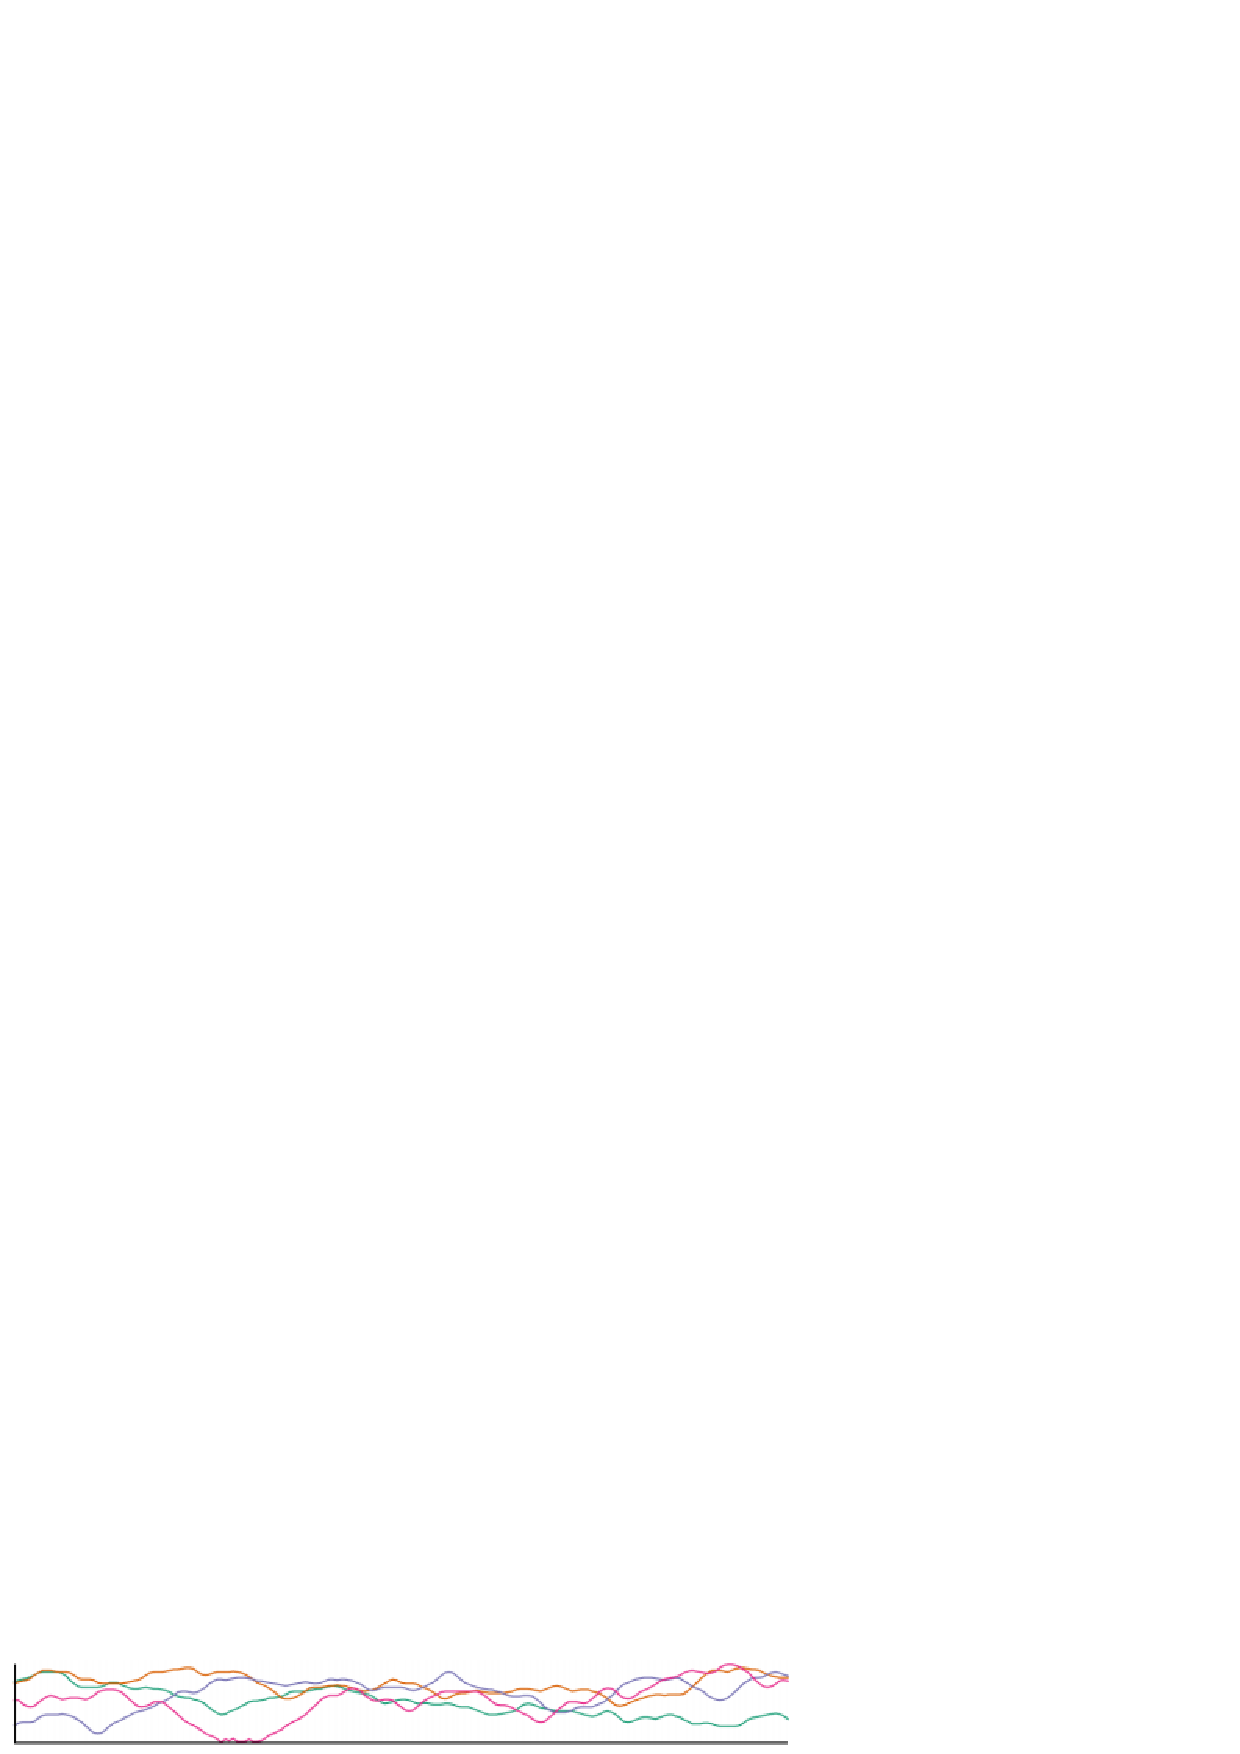
\includegraphics[width=0.48\textwidth]{figures/png/ts_simplelinegraph.png}} 
		\subfigure[A braided graph.]{\label{fig:ts_braid}
\includegraphics[width=0.48\textwidth]{figures/png/ts_braidedgraph.png}} \\
		\subfigure[Small multiples.]{\label{fig:ts_smmult}
\includegraphics[width=0.48\textwidth]{figures/png/ts_smallmultiples.png}}
		\subfigure[Horizon graphs.]{\label{fig:ts_horizon}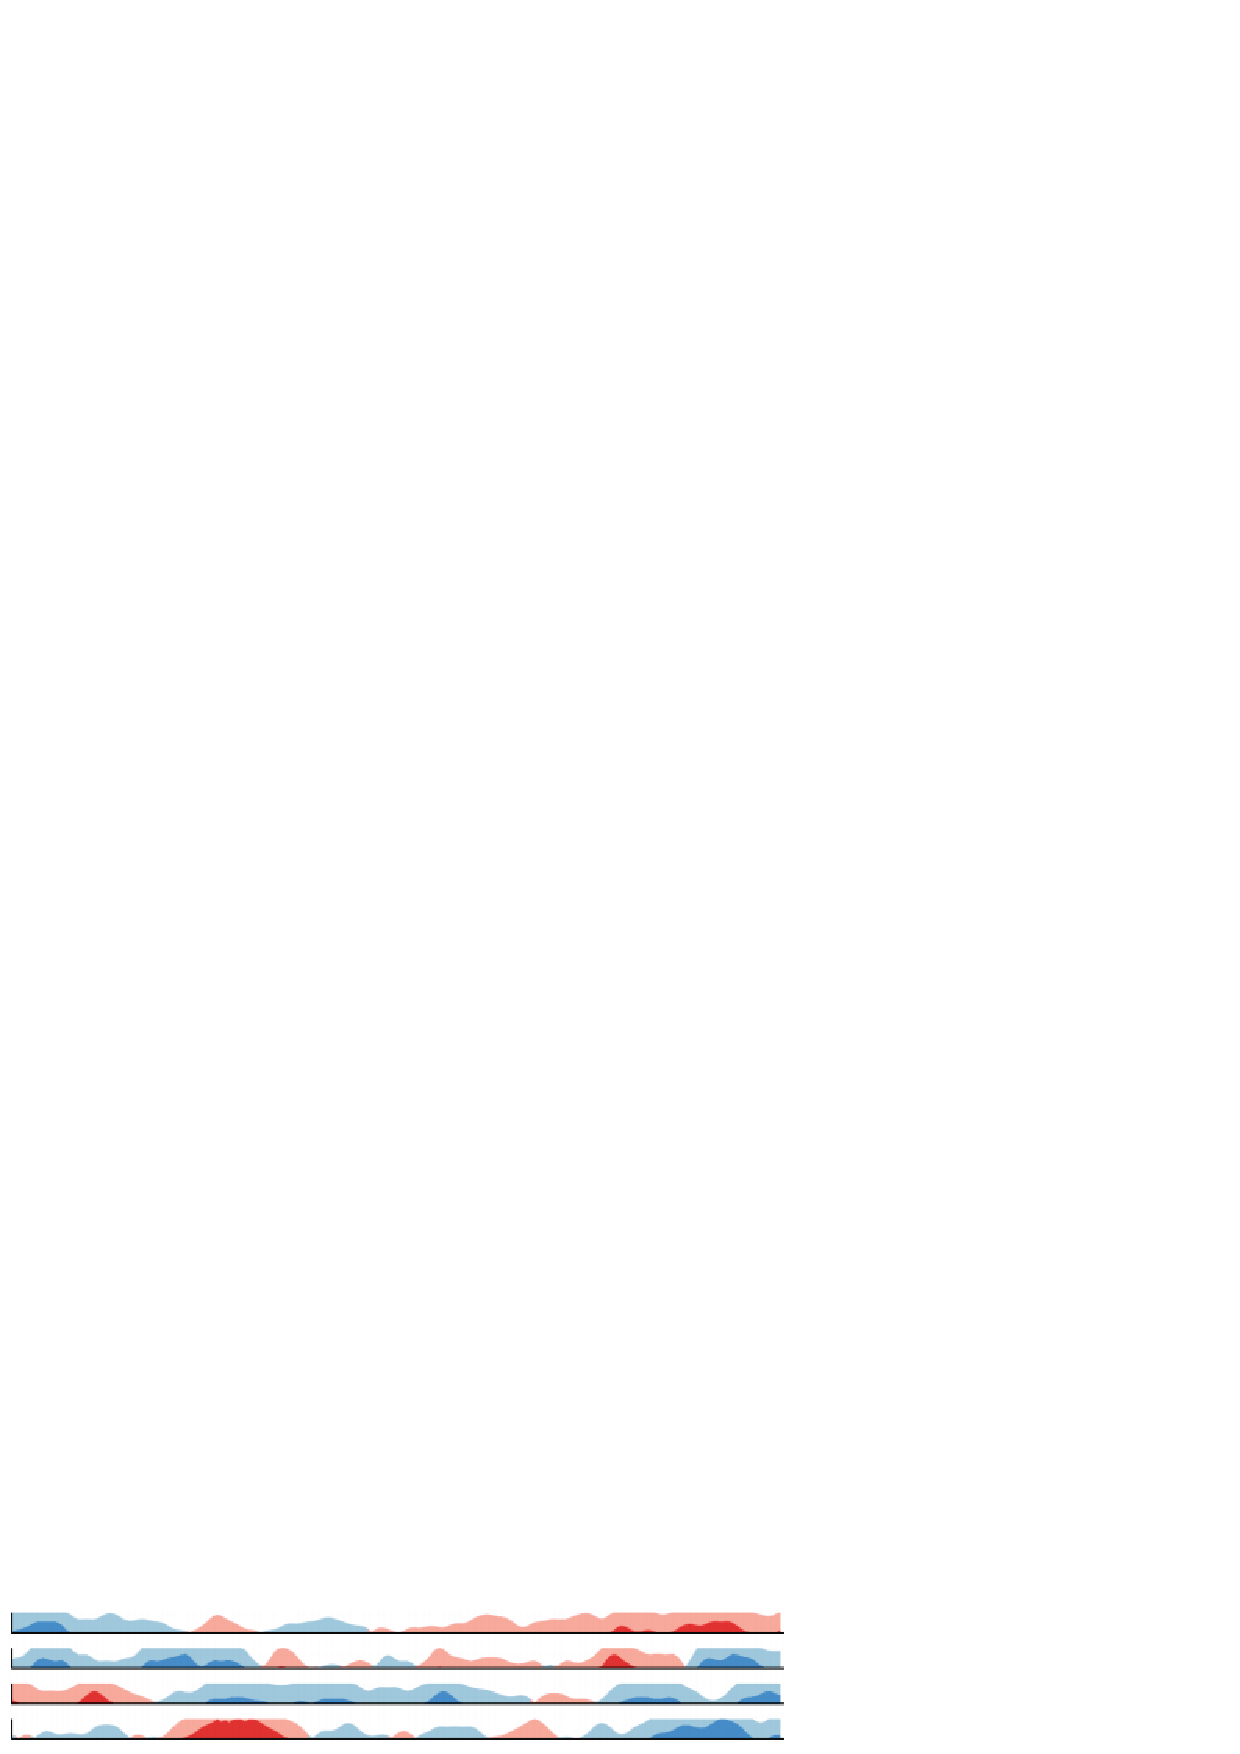
\includegraphics[width=0.48\textwidth]{figures/png/ts_horizongraphs.png}}
	
	\caption[Four possible methods for visualizing multiple time series]{Four possible methods for visualizing multiple time series.  Reprinted from \textit{IEEE Transactions on Visualization and Computer Graphics}, Vol 16, \citeauthor{javed2010}, Graphical perception of multiple time series, 927--934, \textcopyright \citeyear{javed2010}, with permission from IEEE.}

	\label{fig:ts_compare}
\end{figure}

Multiple time series can be part of a single line chart; each series needs only to be distinguished by a color and/or line style.  However, as the number of time series on a single line chart increases, it becomes more difficult to identify an individual series.  Javed et al.\ evaluated the four different plotting techniques for multiple time series illustrated in Figure~\ref{fig:ts_compare} \citeyearpar{javed2010}.  The first of the techniques is the ``simple line chart,'' which is Playfair's original line chart with all series plotted together.  A slight variation on that is ``small multiples,'' where each series has its own line chart though all charts share the same axis scales.  Horizon graphs, originally developed by Saito et al., wrap around a baseline in two color tones to save space \citeyearpar{saitoTwoTone}.  Lastly, braided graphs feature all series on one chart with the coloring under the curves alternating as series intersect each other.  The user evaluation by Javed et al.\ revealed that a simple line graph with all time series on one plot or a single graph for each time series is better suited to a variety of tasks than a horizon graph or a braided graph.  They also found that users complete tasks more correctly when there is more display space allocated to the graphs.  They did not recommend using a higher number of simultaneous time series---their study used eight at the most---because it leads to a decline in correctness of task completion.

\begin{figure}
	\centering
	\subfigure[Shape parameter of 1.0.]{\label{fig:ratioBad}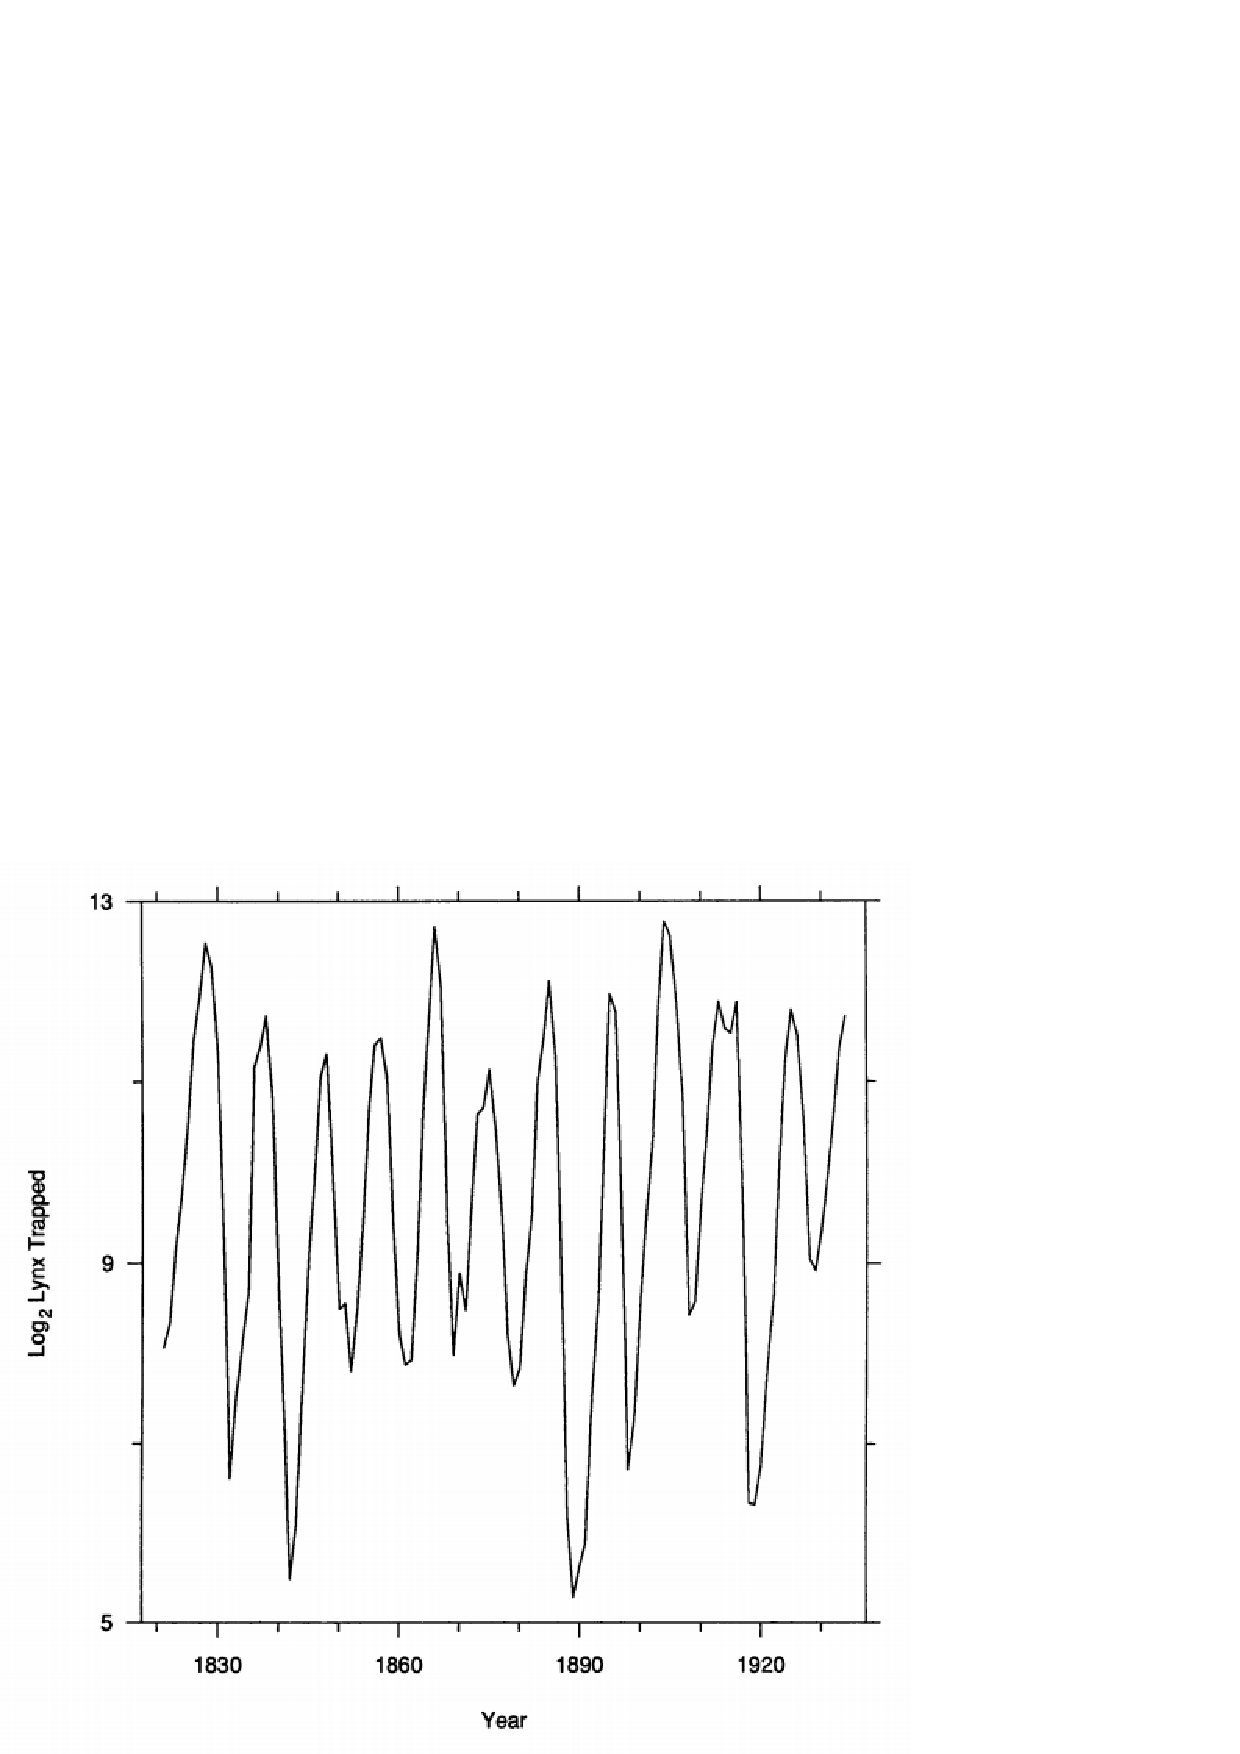
\includegraphics[width=0.45\textwidth]{figures/png/ratioBad.png}} 
	\subfigure[Shape parameter of 0.074.]{\label{fig:ratioGood}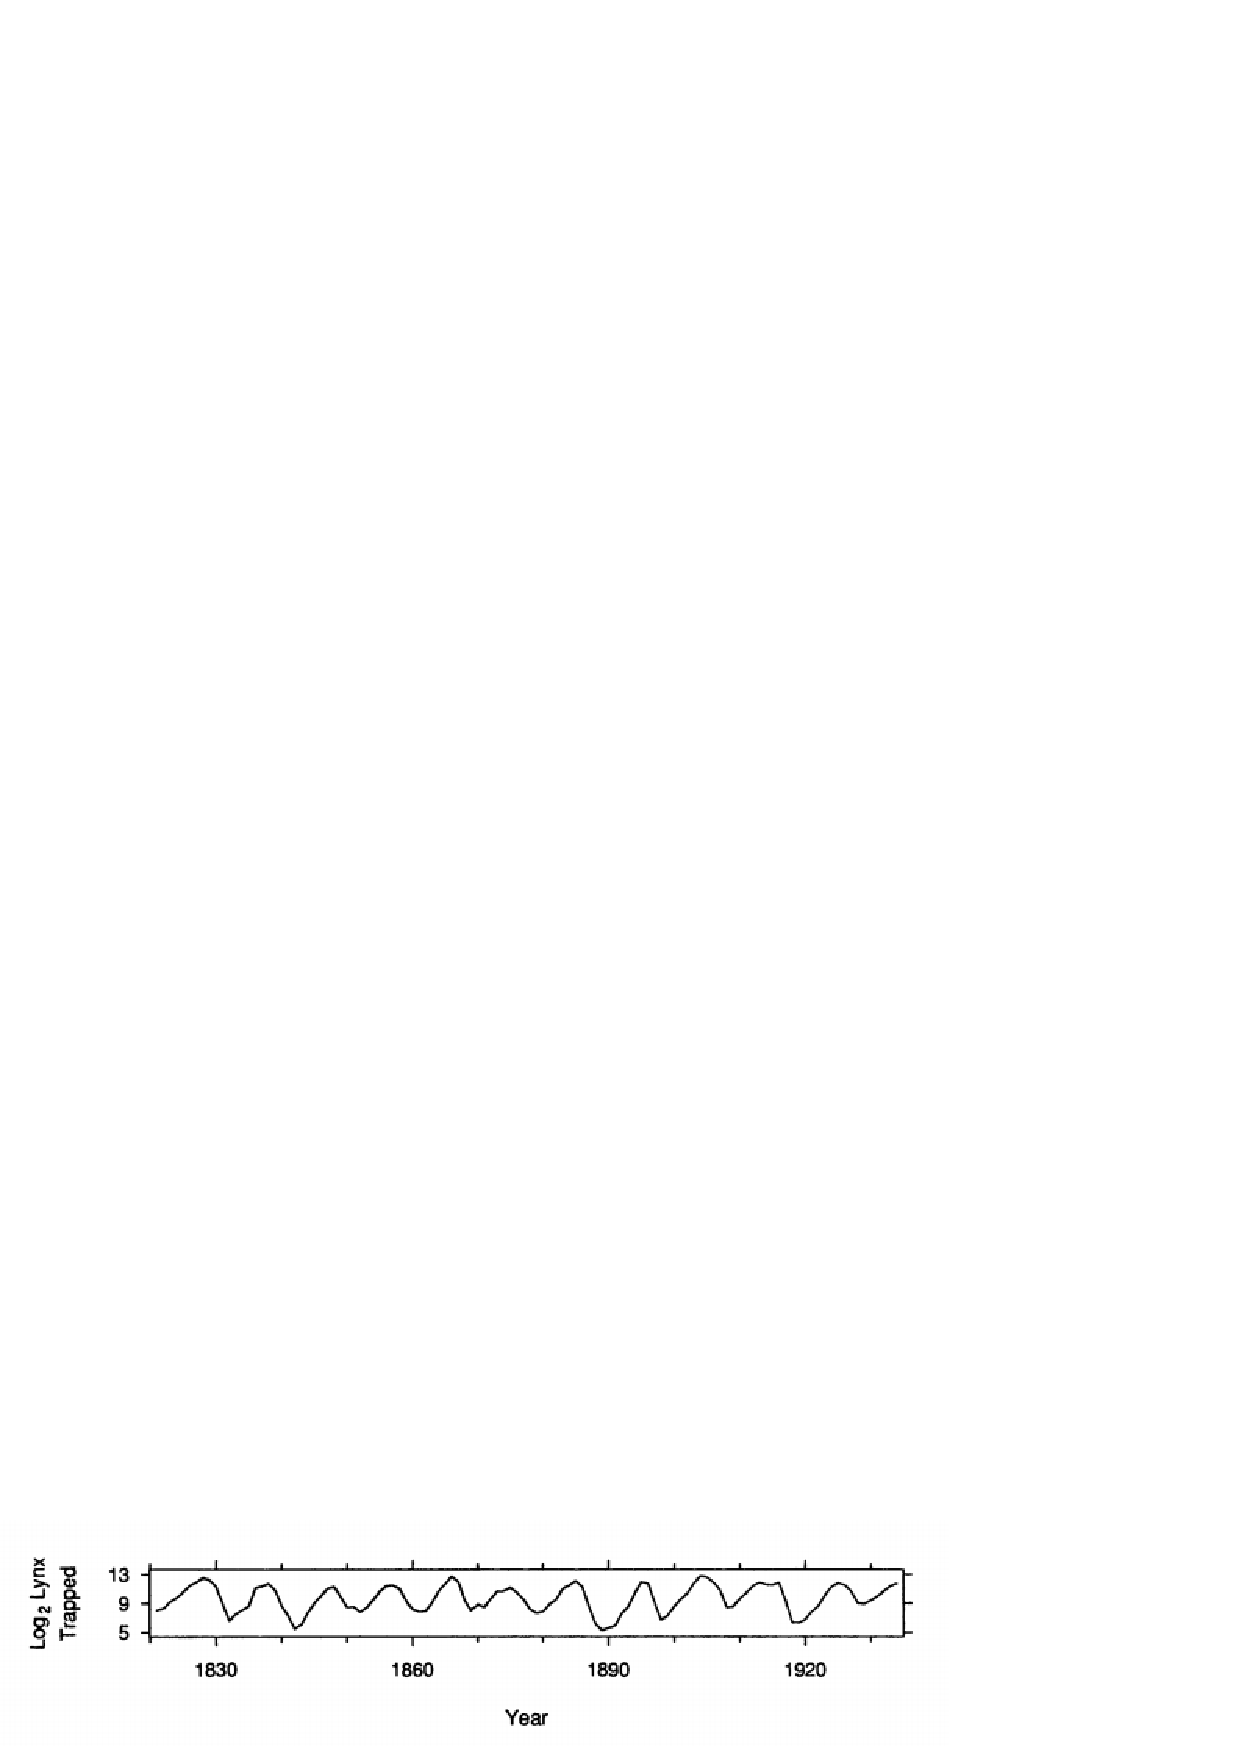
\includegraphics[width=0.45\textwidth]{figures/png/ratioGood.png}}
	\caption[Two effects of chart shape on Canadian lynx data]{Two effects of chart shape on Canadian lynx data.  Reprinted from \textit{Journal of the American Statistical Association}, Vol 83, \citeauthor{cleveland1988}, The Shape Parameter of a Two-Variable Graph, 289--300, \textcopyright \citeyear{cleveland1988}, with permission from Taylor \& Francis.}
	\label{fig:ratio}
\end{figure}

Some line charts are more effective at conveying the nature of the data than others because of the way different drawing techniques affect interpretability.  Cleveland et al.\ found the shape of a line chart---defined as the height of the chart divided by the width of the chart---to be a critical factor \citeyearpar{cleveland1988}.   The shape of the chart directly impacts the slopes of line segments, which viewers interpret in order to understand the dependence of the $y$ variable on the $x$ variable.  Figure~\ref{fig:ratioBad}, a time series of Canadian lynx trapping data, features a shape of 1.0 and seems to imply rapid increases and decreases in the population.  Figure~\ref{fig:ratioGood} features the same data though with a shape of 0.074, which shows more clearly that the population rises somewhat steadily and declines somewhat rapidly, while Figure~\ref{fig:ratioBad} failed to show this.  Their user evaluation found that judgment of two slopes is influenced by the orientation mid-angle, defined as the average of the minimum slope orientation and the maximum slope orientation.  They proposed line chart shape should be selected such that orientations are as close to $\pm 45 ^{\circ}$ as is possible, like in Figure~\ref{fig:ratioGood}.

\begin{figure}
\centering

\subfigure[Spiral time series.  Reprinted from \textit{IEEE Symposium on Information Visualization}, \citeauthor{weber2001}, Visualizing time-series on spirals, 7--13, \textcopyright \citeyear{weber2001}, with permission from IEEE.]{\label{fig:altSpiral}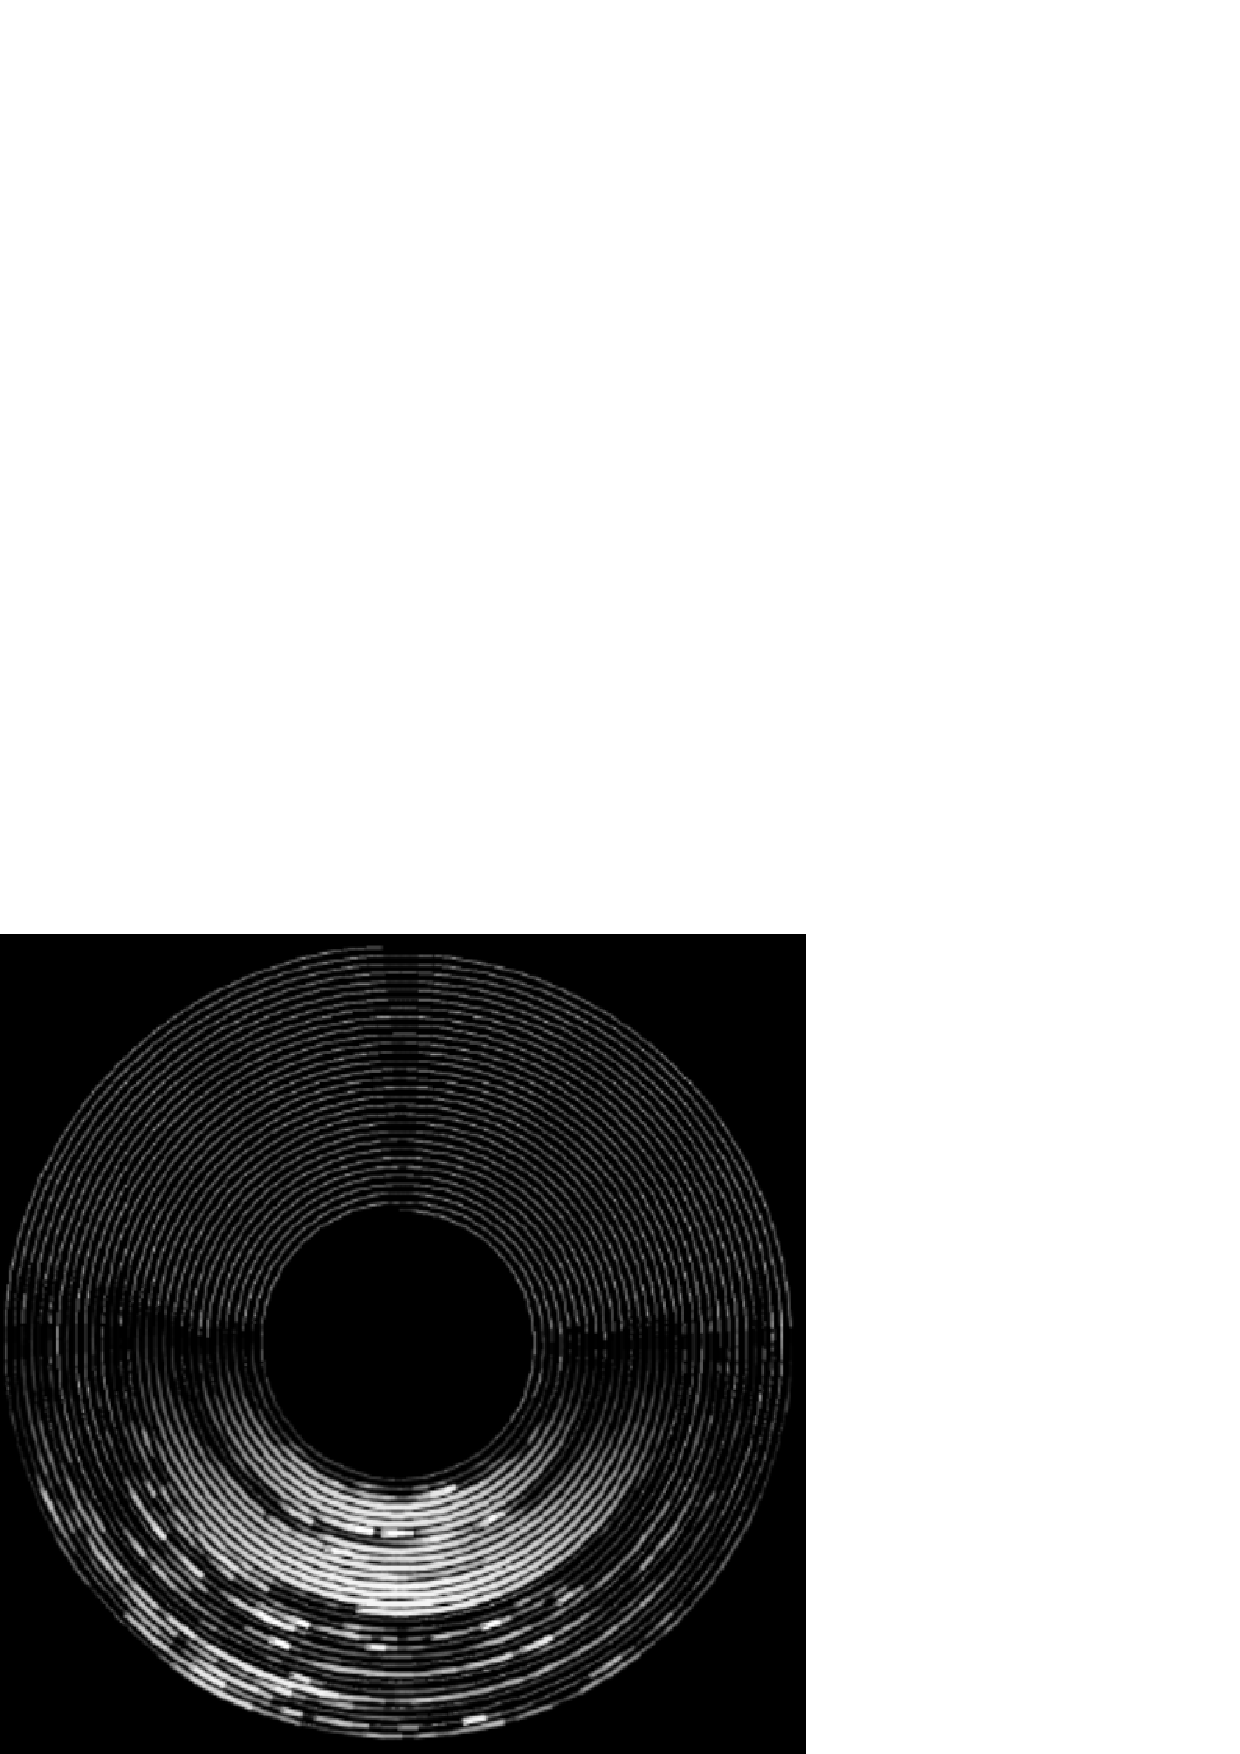
\includegraphics[width=0.45\textwidth]{figures/png/spiral.png}} \qquad
\subfigure[ThemeRiver time series.  Reprinted from \textit{IEEE Symposium on Information Visualization}, \citeauthor{havre2000}, ThemeRiver: visualizing theme changes over time, 115--123, \textcopyright \citeyear{havre2000}, with permission from IEEE.]{\label{fig:altThemeriver}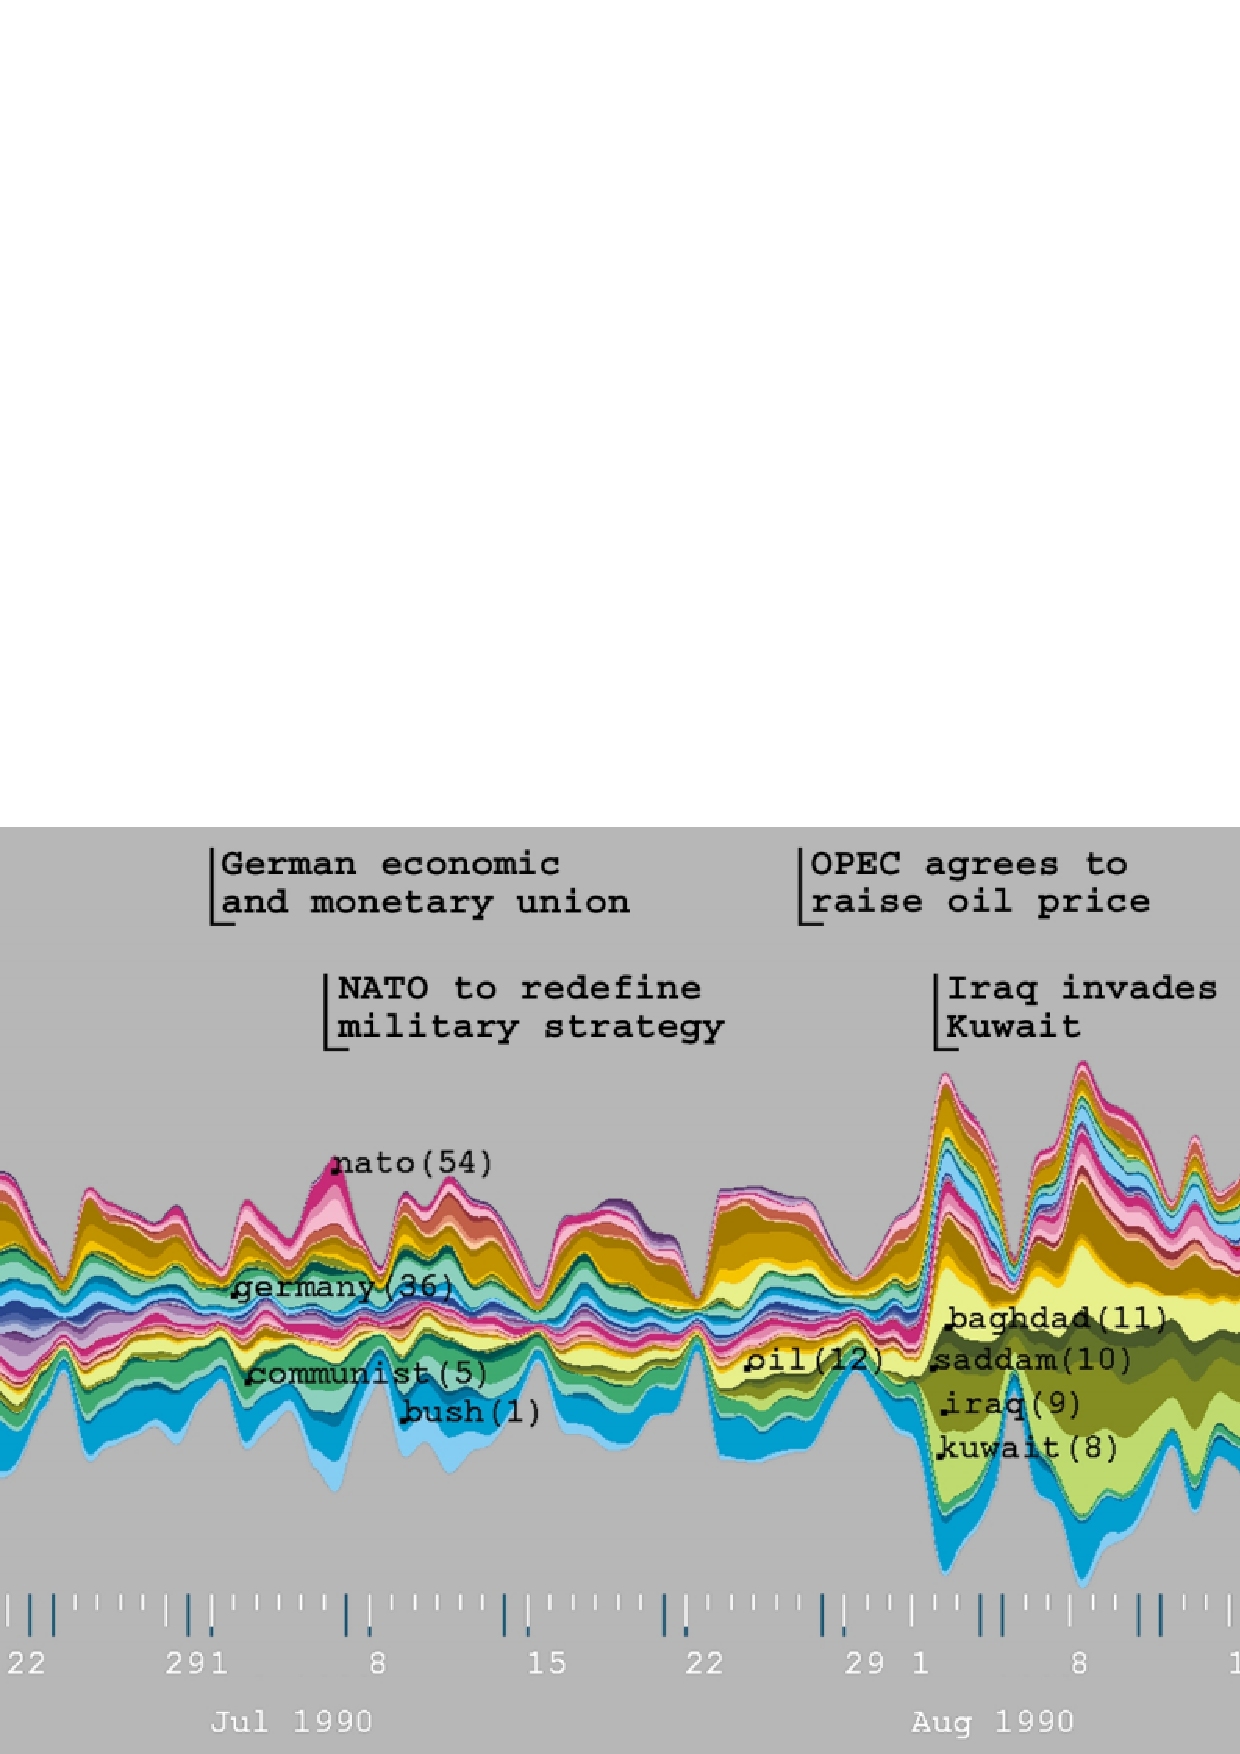
\includegraphics[width=0.45\textwidth]{figures/png/themeriver.png}}

	\caption[Two alternative time series visualizations]{Two alternative time series visualizations.}
	\label{fig:tsAlternatives}
\end{figure}

\subsubsection{Alternatives}

There are many alternatives to and variations of Playfair's original time series.  One example is Weber et al.'s spiral time series, seen in Figure~\ref{fig:altSpiral} \citeyearpar{weber2001}.  The spiral time series was designed for cyclic data.  Cycles are emphasized in a properly-parameterized spiral visualization, however it may be difficult to describe periodic behavior in unknown datasets or determine if that behavior even exists. Another example is the ThemeRiver by Havre et al, seen in Figure~\ref{fig:altThemeriver} \citeyearpar{havre2000}.  Each ``current'' in the ThemeRiver represents an entity or subject and must be of a distinctive color.  Positioning along the y-axis is meaningless, instead the abundance of the entity or subject over time is indicated by the width of the band of color.  The overall width of the stream is the sum of the widths of all individual bands. 

\subsection{Networks}

The input parameters to the MS-PROD model includes predation and competition matrices.  The model may be better understood if these relationships can be incorporated into the visualization. Relationships are often visualized through a node-link diagram, which typically represents entities as nodes and links as relationships between the nodes they connect.  There are many types of node-link diagrams used for illustrating networks; those which are relevant to our research are discussed in the following sections.

\subsubsection{Force-Directed Layouts}

\begin{figure}[h]
	\centering
	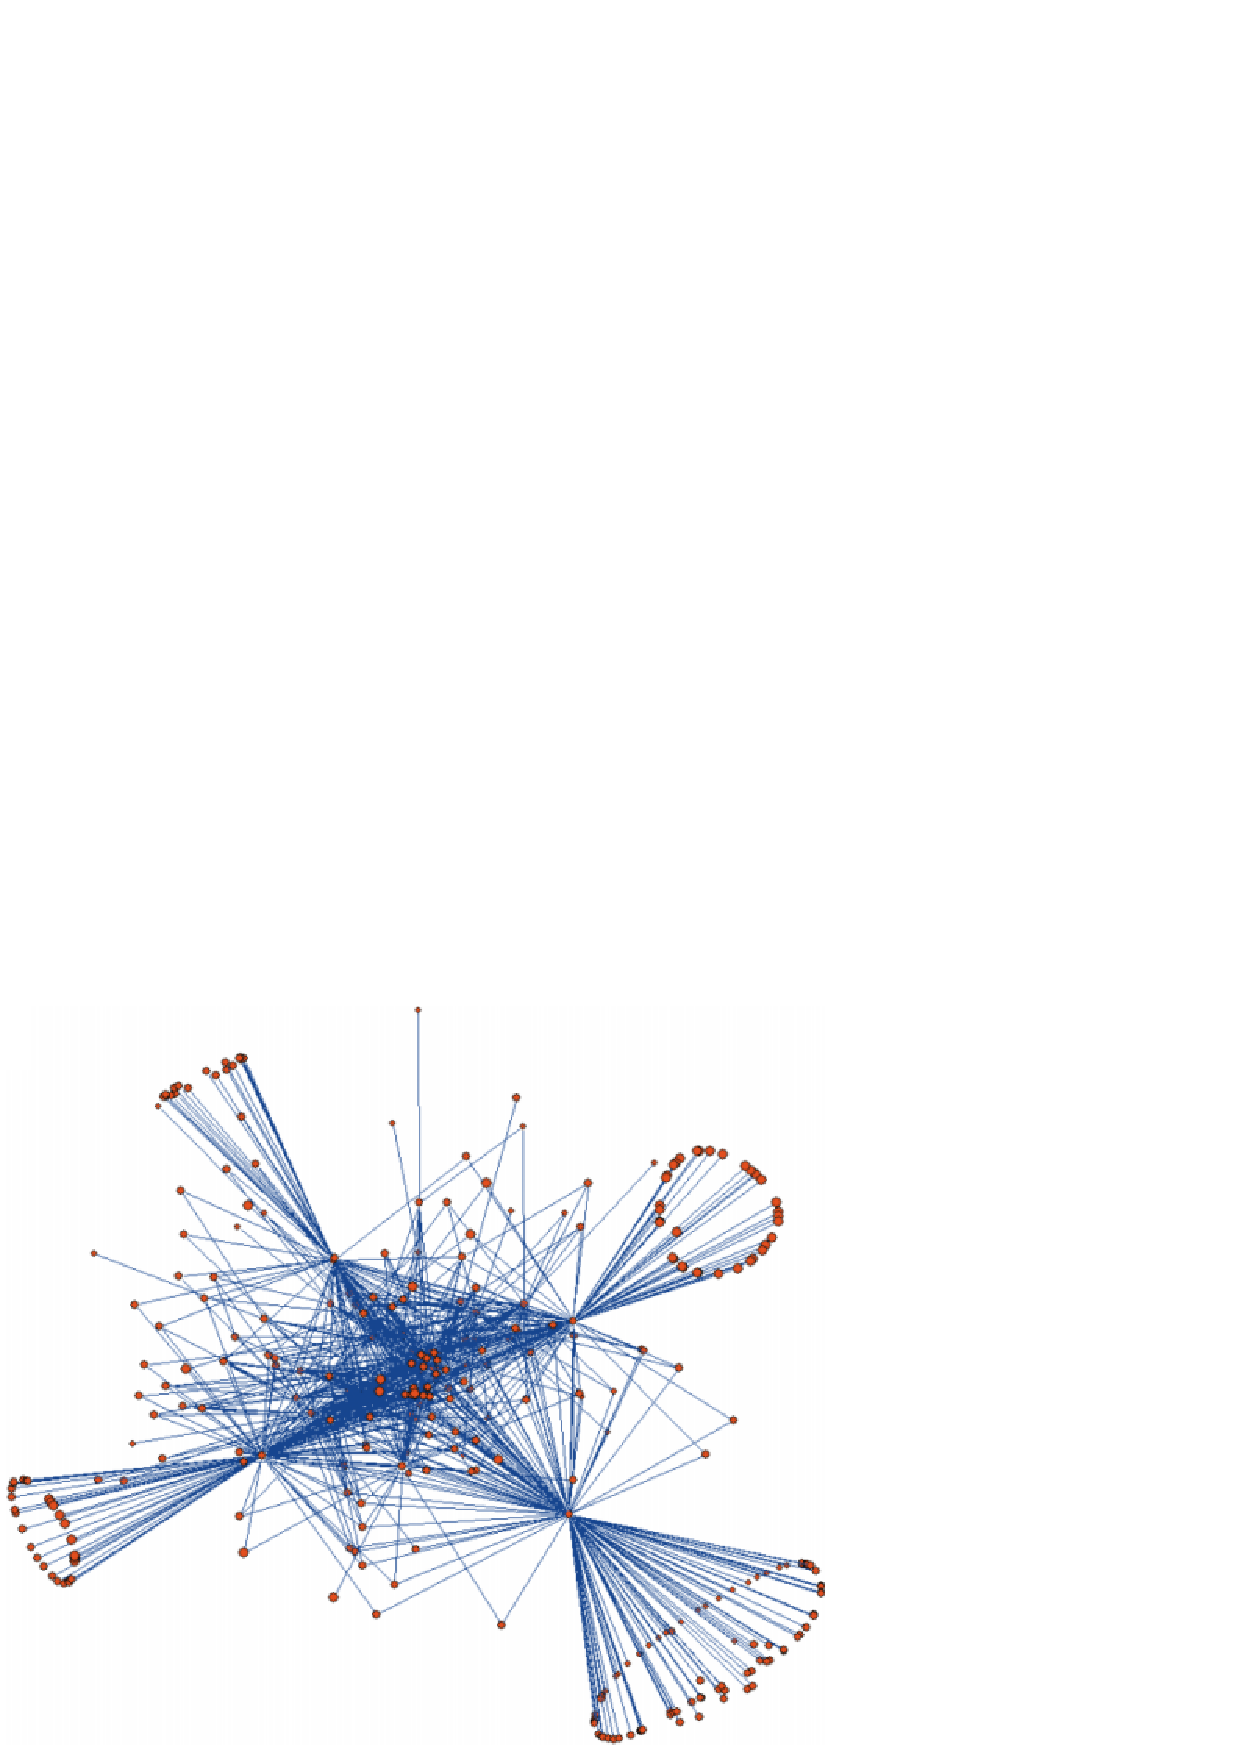
\includegraphics[width=0.85\textwidth]{figures/png/gaichas.png}
	\caption[A force-directed visualization of a food web of Gulf of Alaska data]{A force-directed visualization of a food web of Gulf of Alaska data. Reprinted from \textit{Canadian Journal of Fisheries and Aquatic Sciences}, Vol 65, \citeauthor{gaichas2008}, Network models for ecosystem-based fishery analysis: a review of concepts and application to the Gulf of Alaska marine food web, 129--130, \textcopyright \citeyear{gaichas2008}, with permission from Elsevier.}
	\label{fig:gaichas}
\end{figure}

One option for showing fish species interactions would be to use a force-directed layout as Gaichas and Francis did, seen in Figure~\ref{fig:gaichas} \citeyearpar{gaichas2008}.  Here, the nodes represent an individual species in the Gulf of Alaska, while the links represent a predator-prey interaction.  In a force-directed layout, nodes repel each other, while related nodes become pulled toward each other by links \cite{heer2010}.  The result is an aesthetically pleasing layout where there are relatively few link crossings and links are of approximately similar length.  The color of the node can be used to indicate group membership, while the size can represent the magnitude of some property of the node.  Likewise, the drawing style of the link can be varied to encode different types of relationships.  Depending on the size of the network, a force-directed layout can be dense, as shown in Figure~\ref{fig:gaichas}, making it difficult to discern individual nodes or links.  Interactive methods can alleviate this by allowing the user to zoom or to click a node and see only the subset of the network directly connected to that node.

\subsubsection{Arc Diagrams}

\begin{figure}[h]
	\centering
	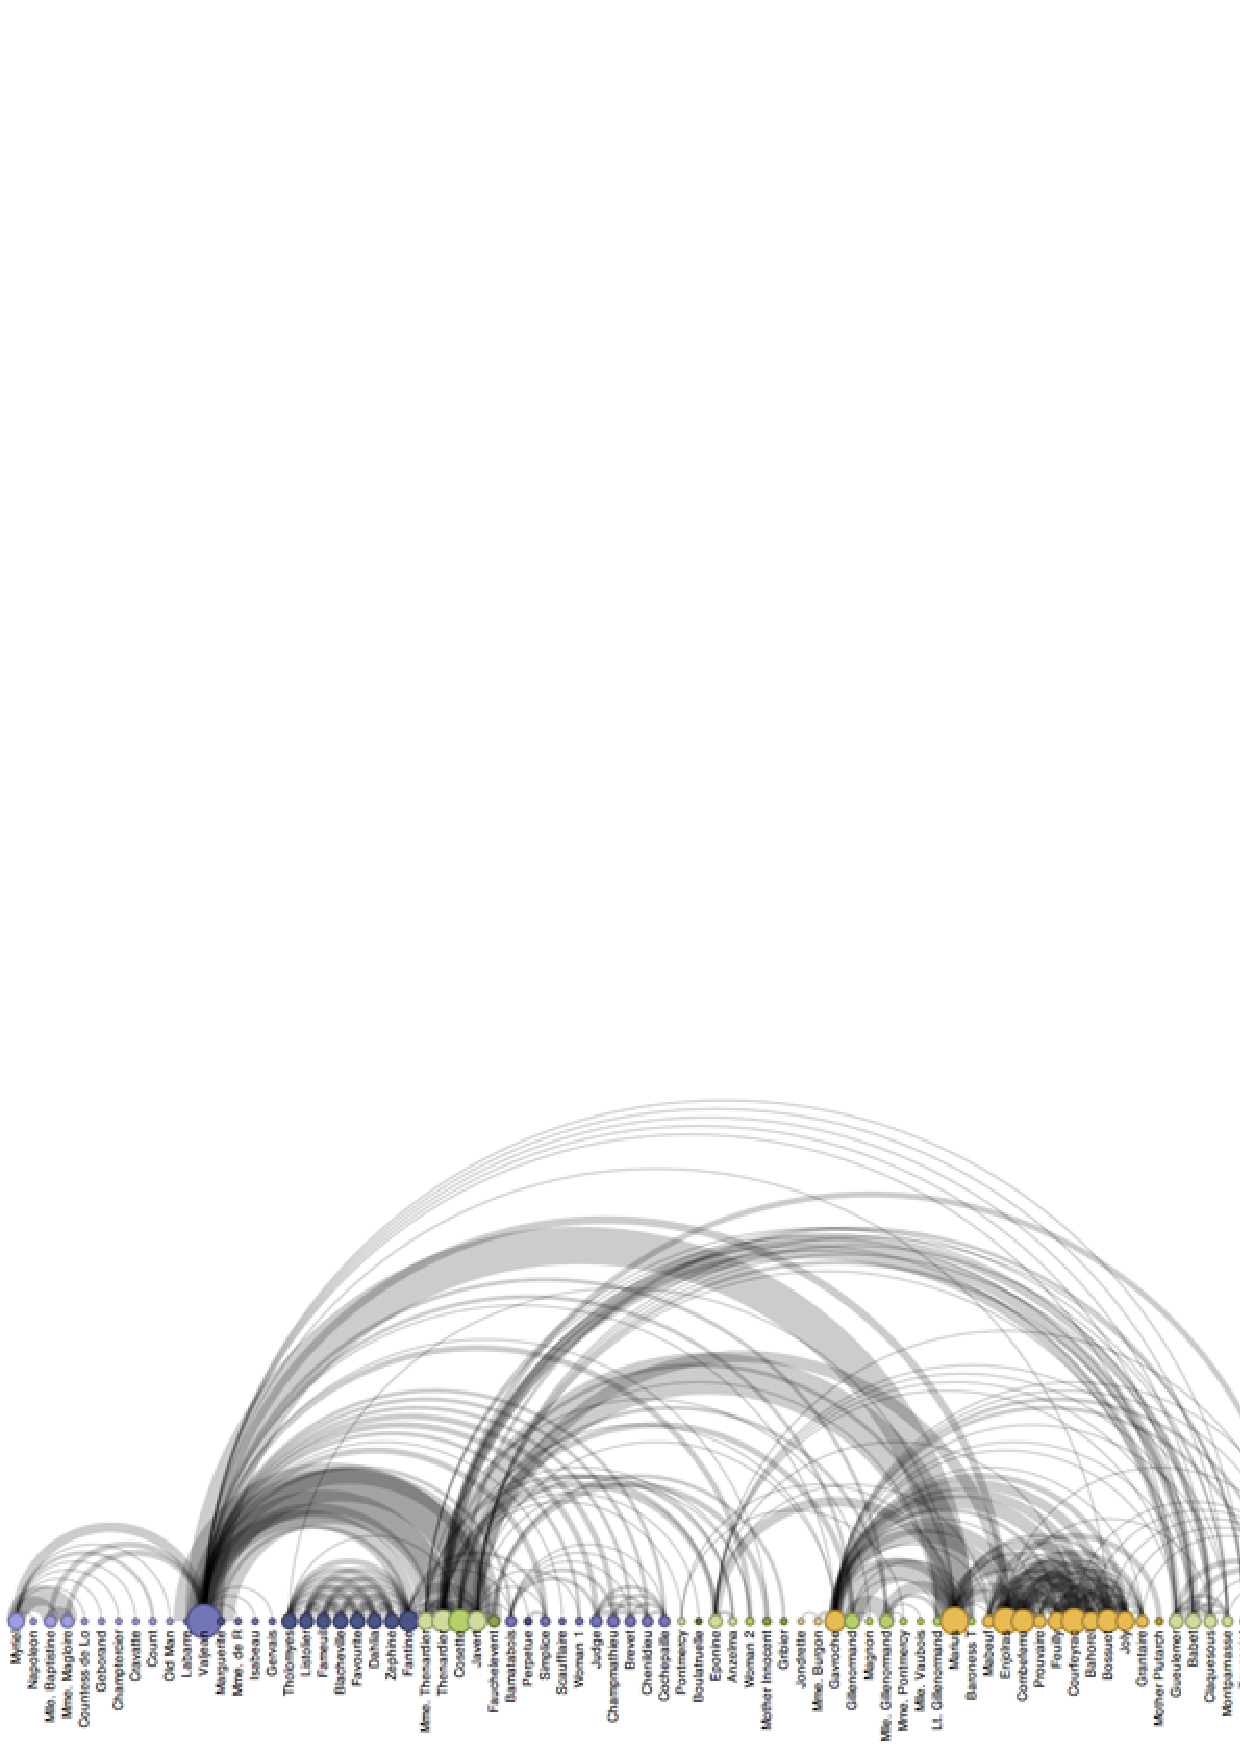
\includegraphics[width=0.95\textwidth]{figures/png/arcdiagram.png}
	\caption[Knuth's arc diagram of \textit{Les Mis\'erables} characters]{Knuth's arc diagram of \textit{Les Mis\'erables} characters.  Image reproduced with permission from Jeffrey Heer.}
	\label{fig:arcdiagram}
\end{figure}

An alternative for force-directed layout is an arc diagram.  The name arc diagram was coined by Wattenberg \citeyearpar{wattenberg2002}, though they were invented earlier.  Knuth used arc diagrams to illustrate interaction of characters in Victor Hugo's novel \textit{Les} \textit{Mis\'erables}, seen in Figure~\ref{fig:arcdiagram} \citeyearpar{knuth1993}.  Each character is represented with a circular node, where size indicates the number of appearances in the novel.  The nodes are arranged linearly, colored and ordered according to clusters of characters that appear together frequently.  Semi-transparent arcs are drawn between the characters who appear in the same chapter, with the thickness of the arc representing the number of such appearances.  While the arc diagram may fail to properly depict the structure of a network, Heer et al.\ point out it is advantageous because the one-dimensionality allows for other features to be easily displayed near the nodes \citeyearpar{heer2010}, such as text labels.

\subsubsection{Directed Edges}

\begin{figure}[h]
	\centering
	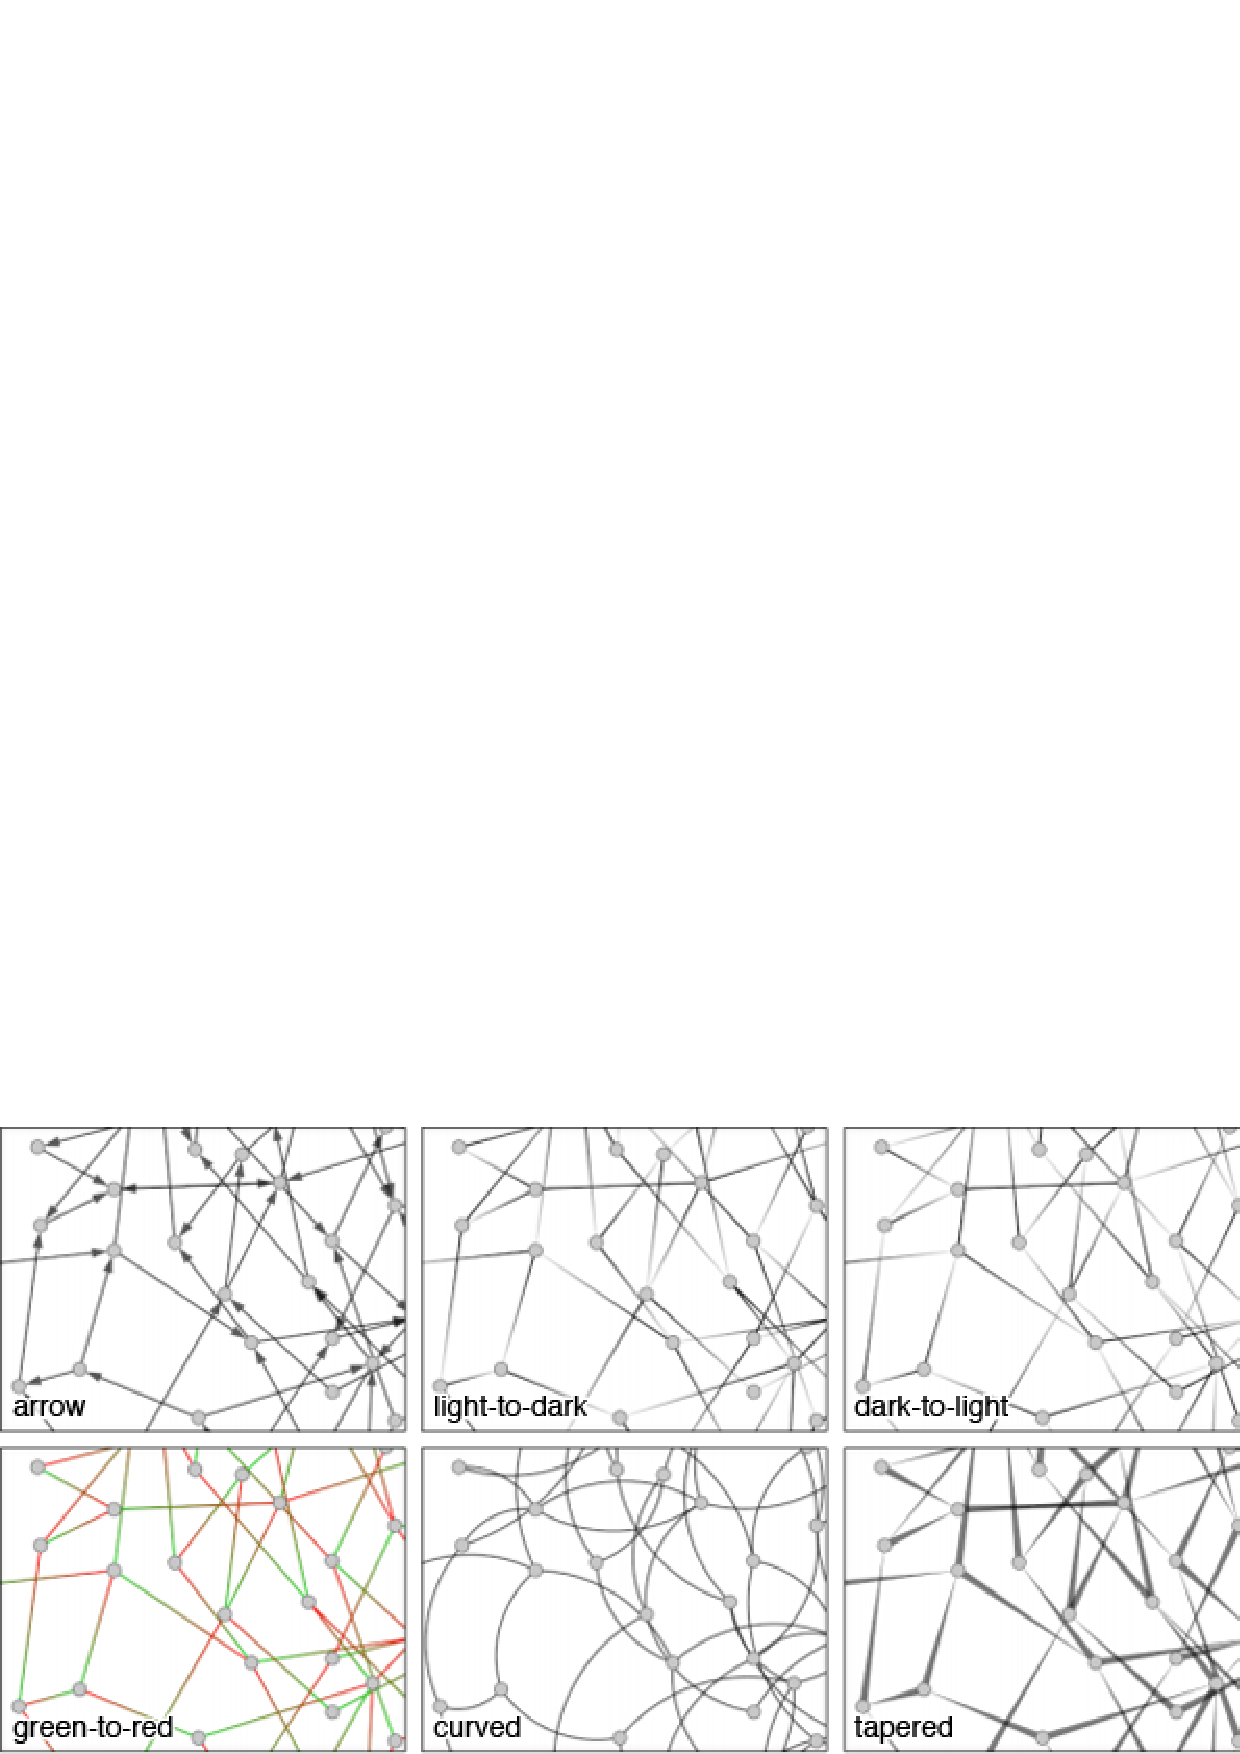
\includegraphics[width=0.95\textwidth]{figures/png/directedEdges.png}
	\caption[Different types of directed edges]{Different types of directed edges.}
	\label{fig:directedEdges}
\end{figure}

Relationships in a network may be directional, such as the predator-prey relationship.  In a visualization of such a network, the direction of the edges must be encoded so these relationships can be understood.  Holten and van Wijk studied the effectiveness of different techniques for indicating directionality of edges in a graph, seen in Figure~\ref{fig:directedEdges} \citeyearpar{holten2009}.  The traditional arrowhead was found to perform poorly, while tapered edges performed best.  As for an intensity-based direction cue, a dark-to-light representation was found to be clearer than light-to-dark.

\subsubsection{Matrix Representations}

\begin{figure}[h]
	\centering
	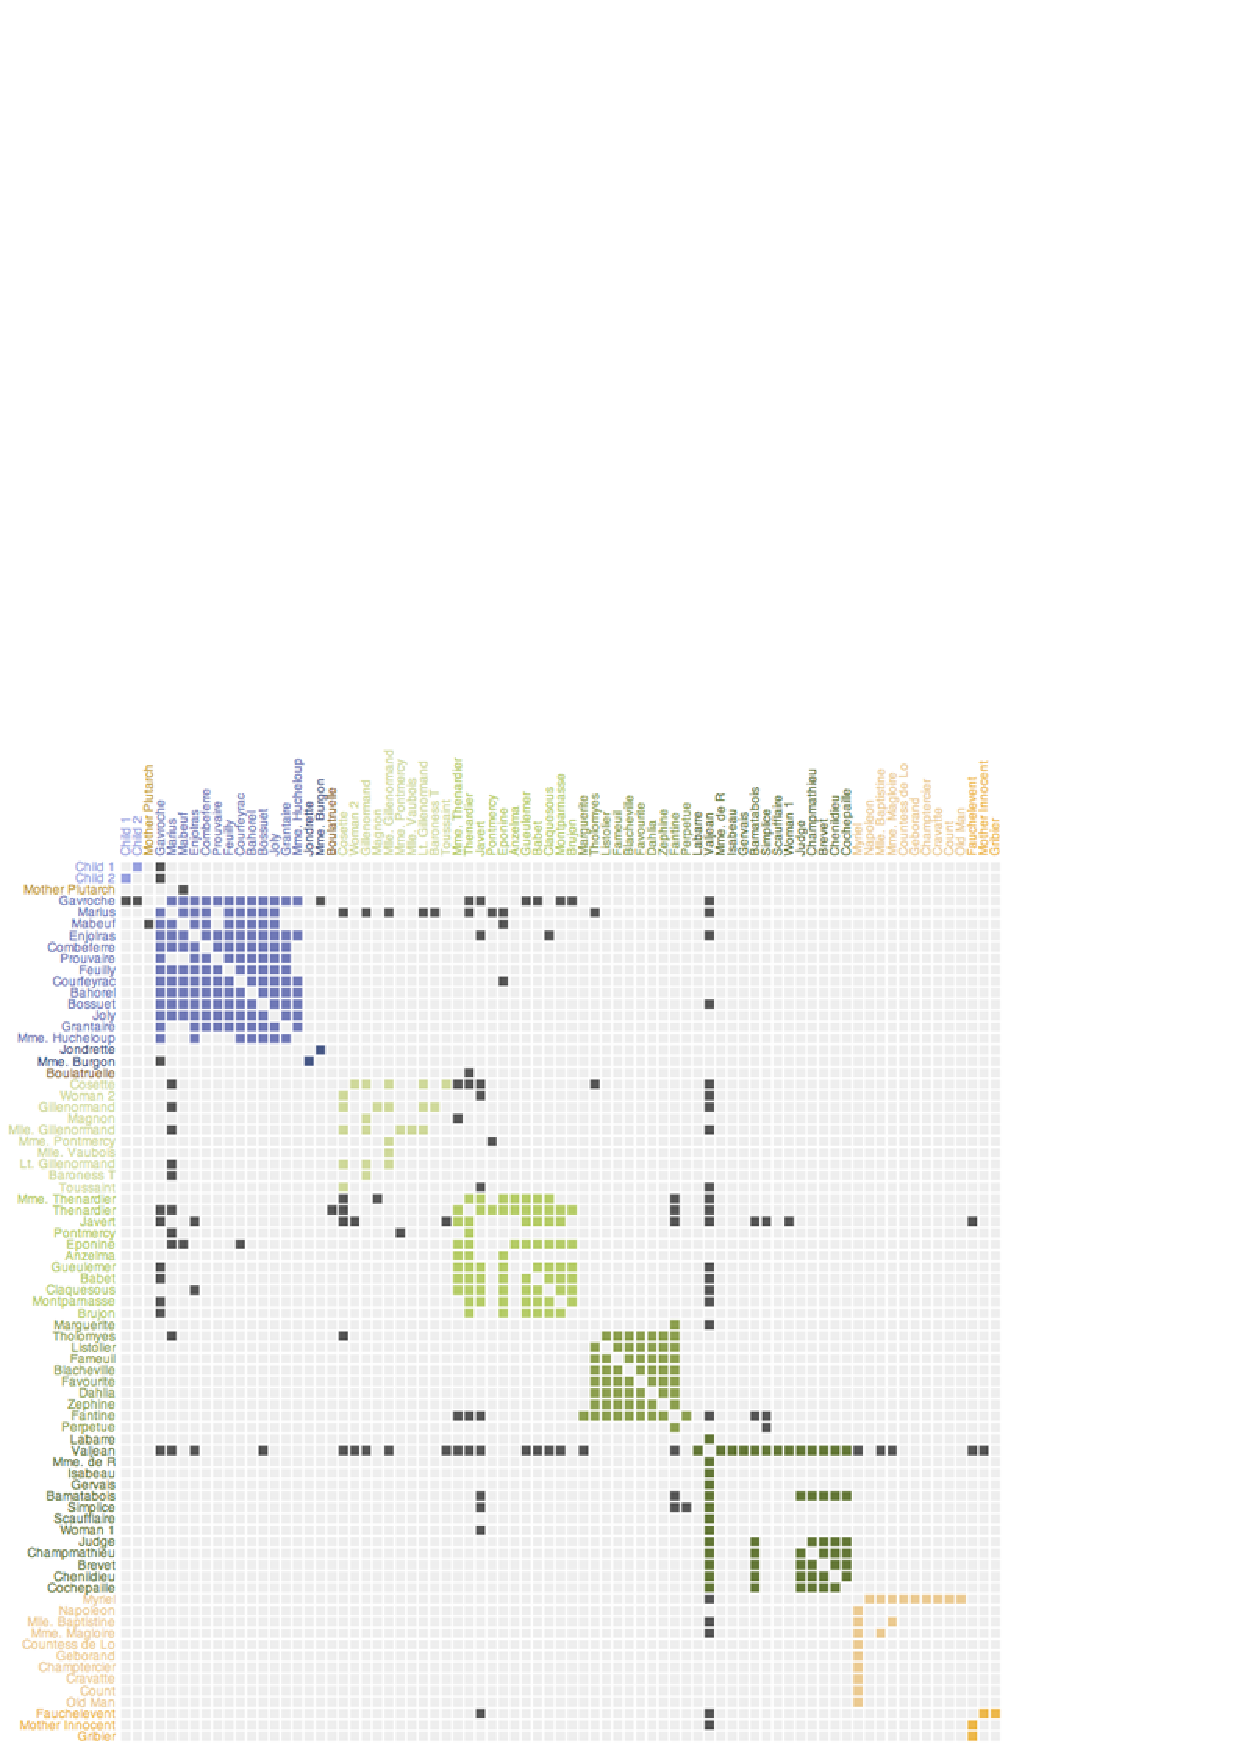
\includegraphics[width=0.95\textwidth]{figures/png/matrix.png}
	\caption[A matrix-based visualization of an adjacency matrix]{A matrix-based visualization of an adjacency matrix.  Image reproduced with permission from Jeffrey Heer.}
	\label{fig:matrix}
\end{figure}

Node-link diagrams can have occlusion problems when they are highly-connected, so a matrix-based representation of a network is a possible alternative \cite{heer2010}.  In many cases, networks are stored as an adjacency matrix, so all that needs to be done is visualize that matrix as a grid, where the cell at the $i$th row and the $j$th column represents the relationship from entity $i$ to entity $j$.  Figure~\ref{fig:matrix} shows Knuth's visualization of \textit{Les} \textit{Mis\'erables} characters in matrix-form \cite{knuth1993}.  The color of the cell indicates the presence or type of a relationship, with some neutral color indicating the lack of a relationship.  Ghoniem et al.\ showed that a matrix-based view is suitable for large or dense networks for tasks that involve finding or counting links or nodes \citeyearpar{ghoniem2004}.  With proper ordering of the rows and columns, the structure of the network can be effectively displayed, however path-finding tasks may be difficult.

\subsection{Causality}

Gamble and Link found that both inter-species relationships and harvesting by humans can contribute to changes in species biomass according to their MS-PROD model \cite{gamble2009}.  For example, an increase in biomass for one species could possibly hinder growth for another species.  Because this is a type of cause and effect relationship, it is necessary to consider the various techniques for representing causality in a network, especially in an interactive context.

\begin{figure}
\centering

\subfigure[Pinball.]{\label{fig:vcvPinball}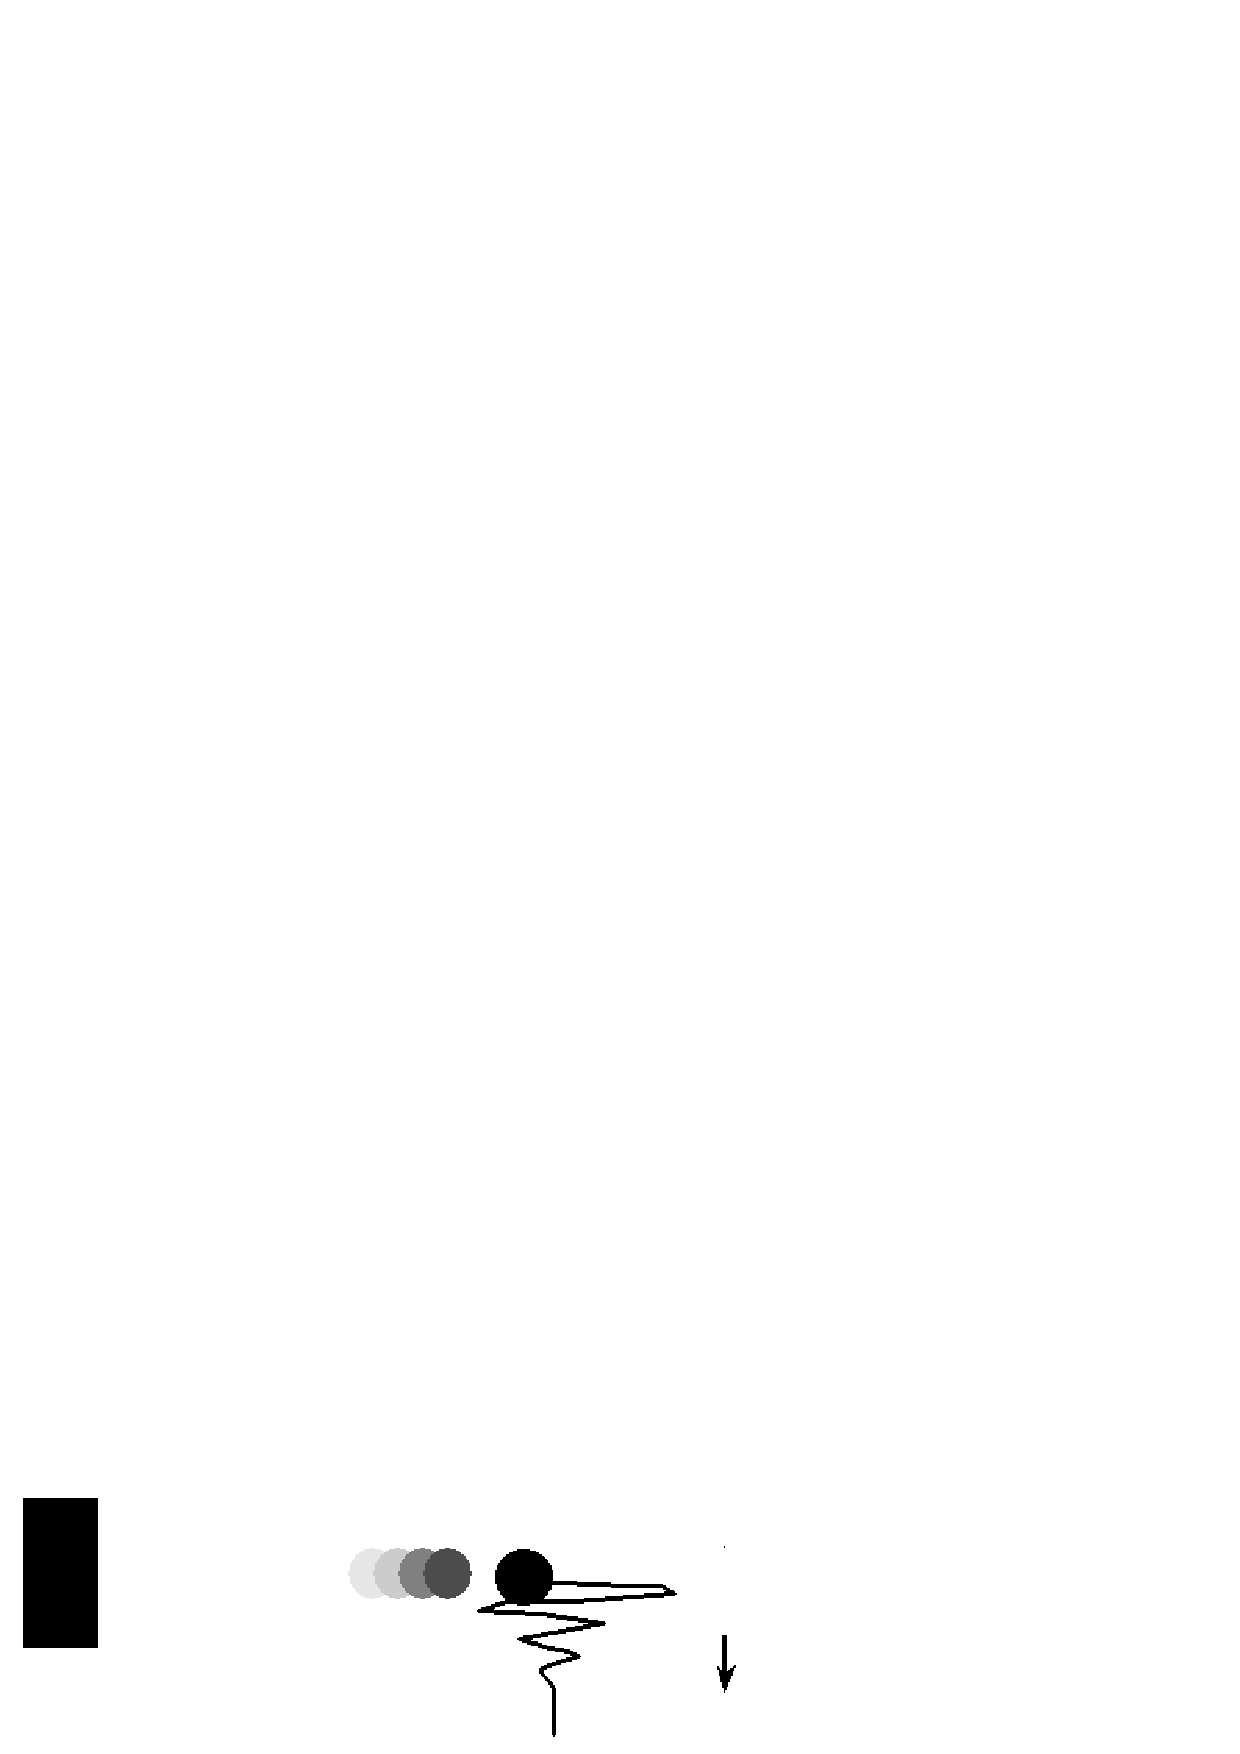
\includegraphics[width=0.31\textwidth]{figures/png/vcv_pinball.png}} 
\subfigure[Prod.]{\label{fig:vcvProd}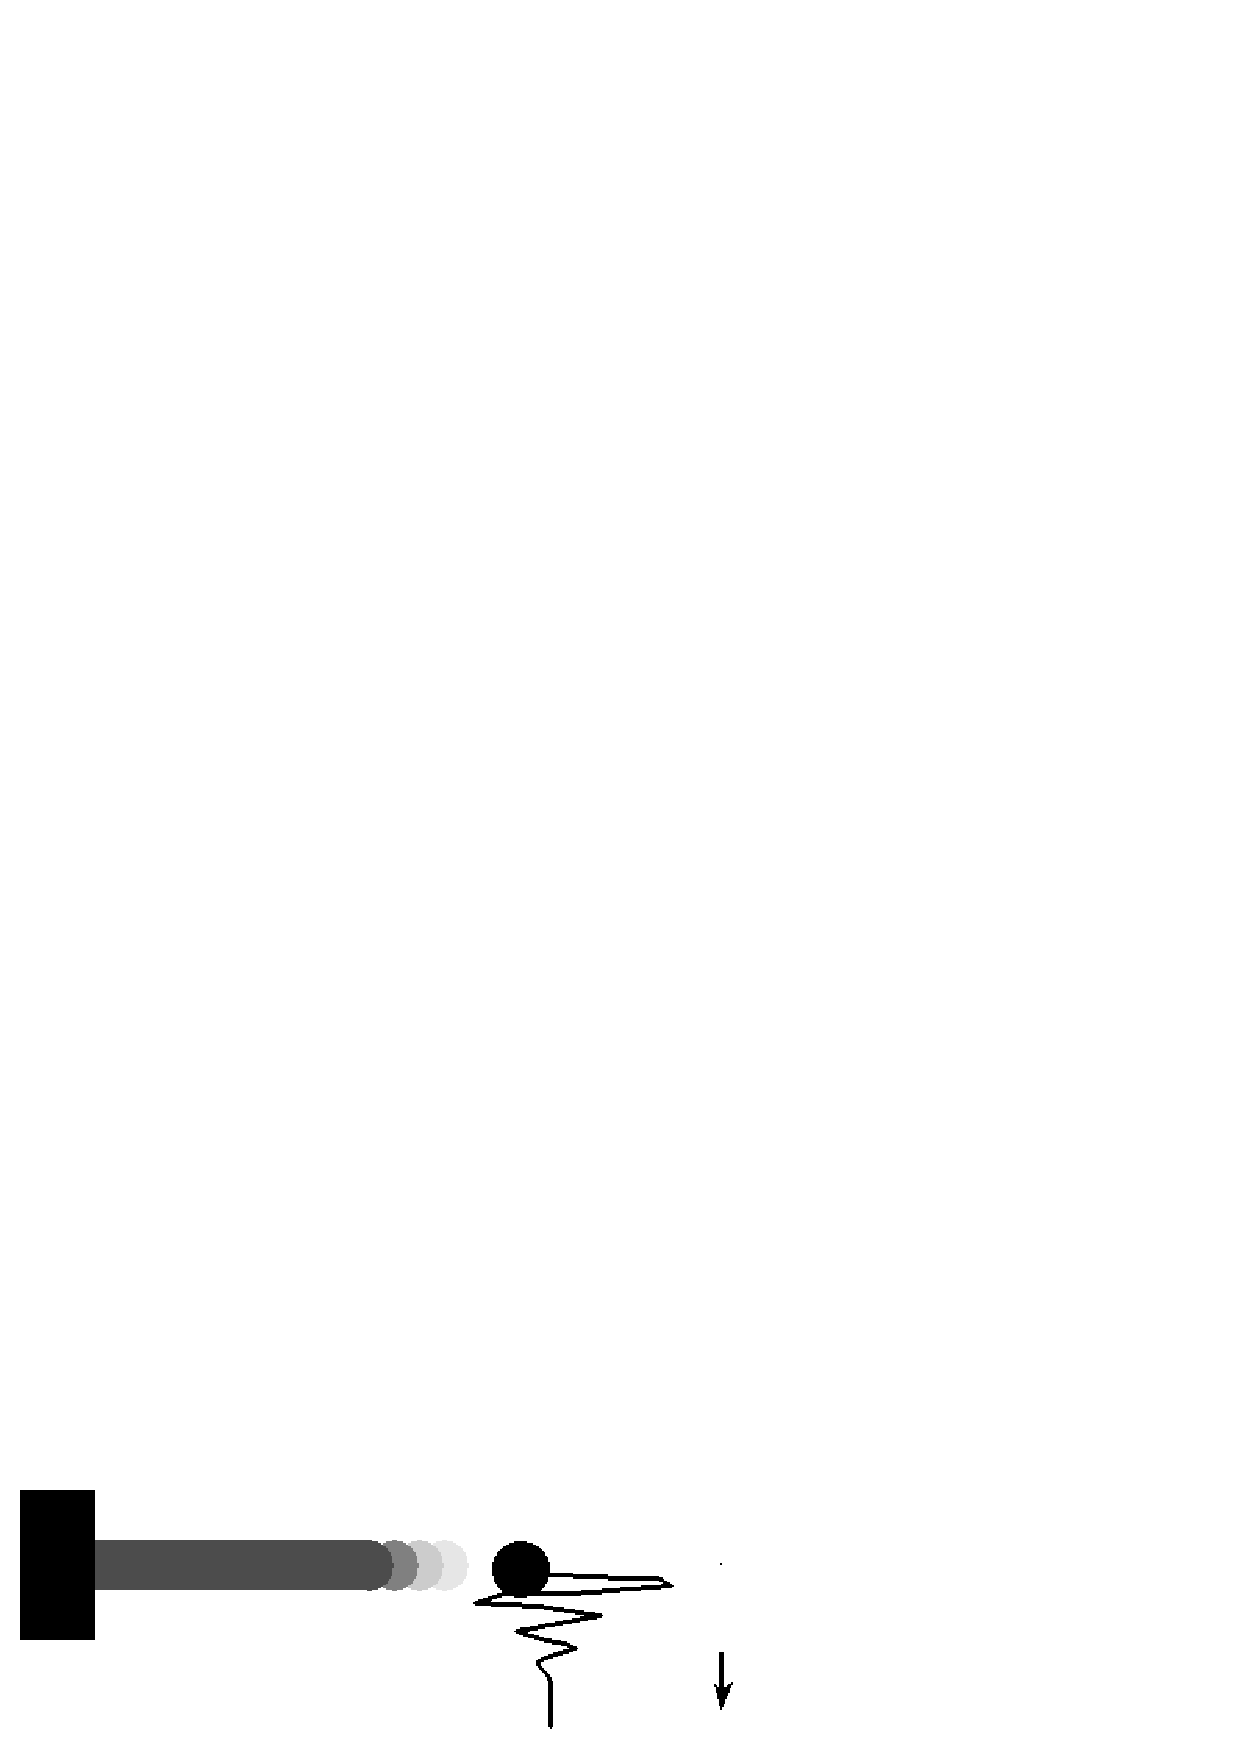
\includegraphics[width=0.31\textwidth]{figures/png/vcv_prod.png}} 
\subfigure[Wave.]{\label{fig:vcvWave}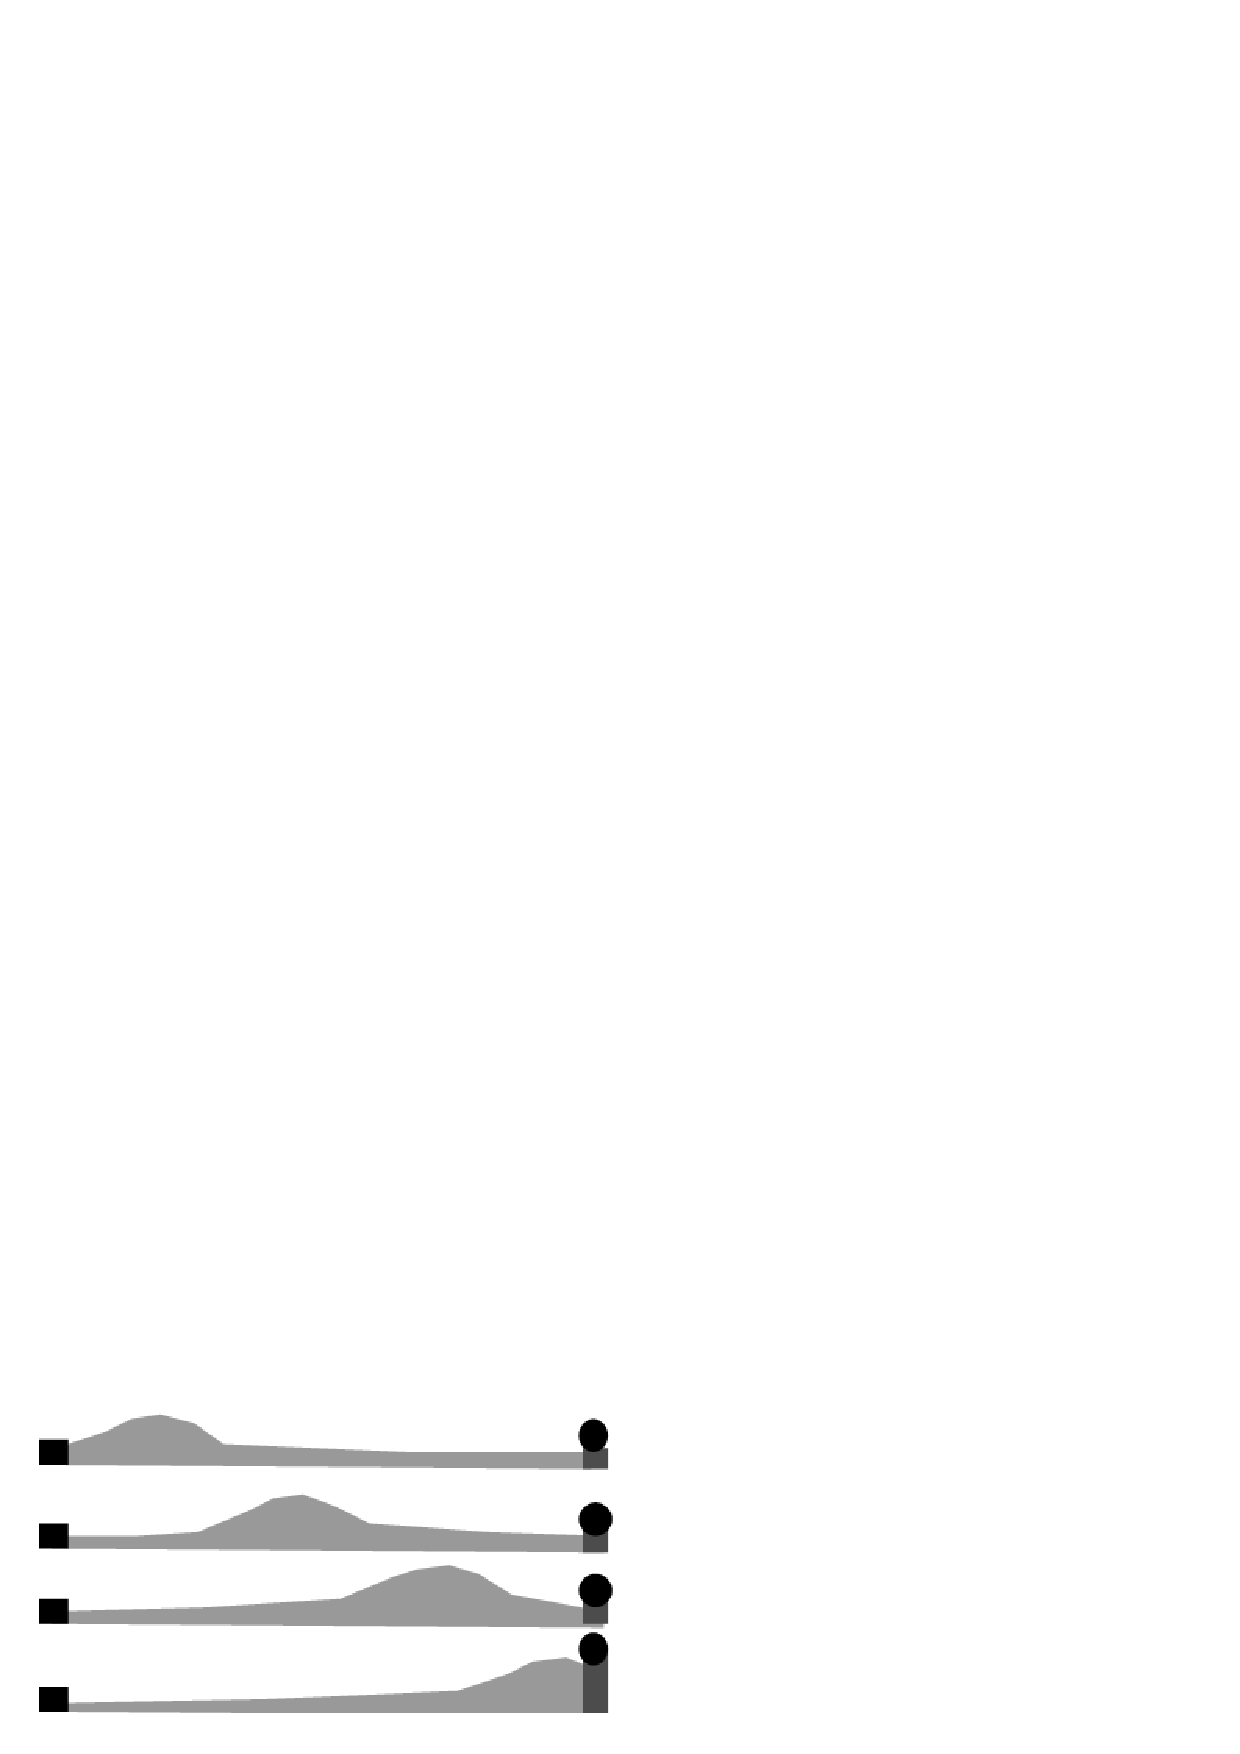
\includegraphics[width=0.31\textwidth]{figures/png/vcv_wave.png}}

\caption[Three metaphors for conveying causality]{Three metaphors for conveying causality.  Reprinted from \textit{IEEE Symposium on Information Visualization: Late Breaking Hot Topics}, \citeauthor{ware1999}, Visualizing causal relations, 39--42, \textcopyright \citeyear{ware1999}, with permission from IEEE.}

	\label{fig:vcv}
\end{figure}

Michotte and Thin\'es suggested that viewers infer causality when viewing an object being set into motion after being struck by another object \citeyearpar{michotte1963}.  This served as a basis for Ware et al.'s visual causality vector (VCV), which communicates causal relationships between two nodes in a network visualization \citeyearpar{ware1999}.  They studied how several animated metaphors---shown in Figure~\ref{fig:vcv}---and different timing rules for a VCV affect the perception of causality.  Their evaluation showed that temporal synchrony between the animation of the metaphor and the changes in the recipient node is more critical than the type of metaphor for showing causal relationships.  Ware later revisited this work in the context of multi-touch screens to convey causal effect enhancements, causal effect reductions, and causal blocking effects using colored pulses \citeyearpar{ware2013}.  The user evaluation conducted by Ware showed that causal blocking effects and positive enhancements were well understood with this design, while negative causal effects were less reliably judged.  Still, these methods were recommended for showing simple causal relationships.

\begin{figure}
\centering
\subfigure[Static.]{\label{fig:kadabaStatic}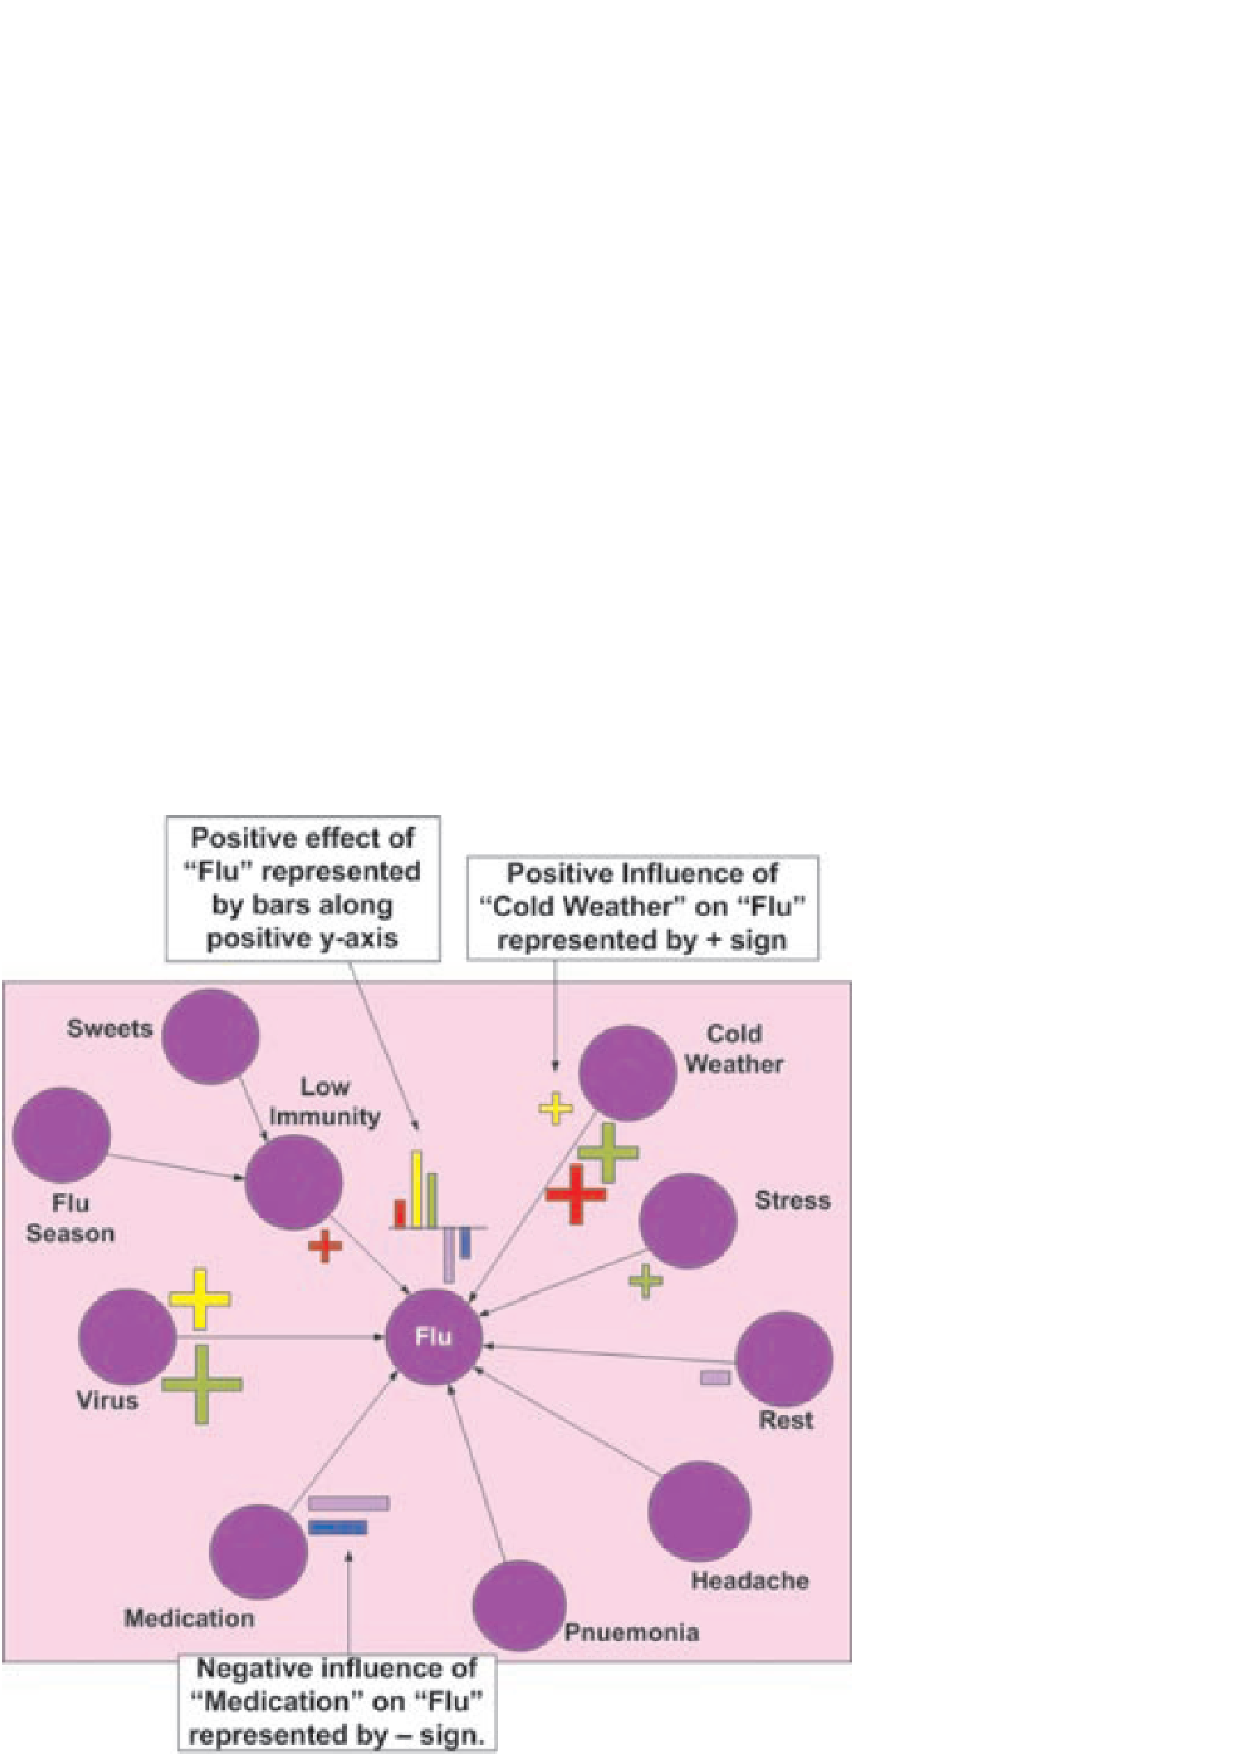
\includegraphics[width=0.46\textwidth]{figures/png/kadaba_static.png}} 
\subfigure[Animated.]{\label{fig:kadabaAnimated}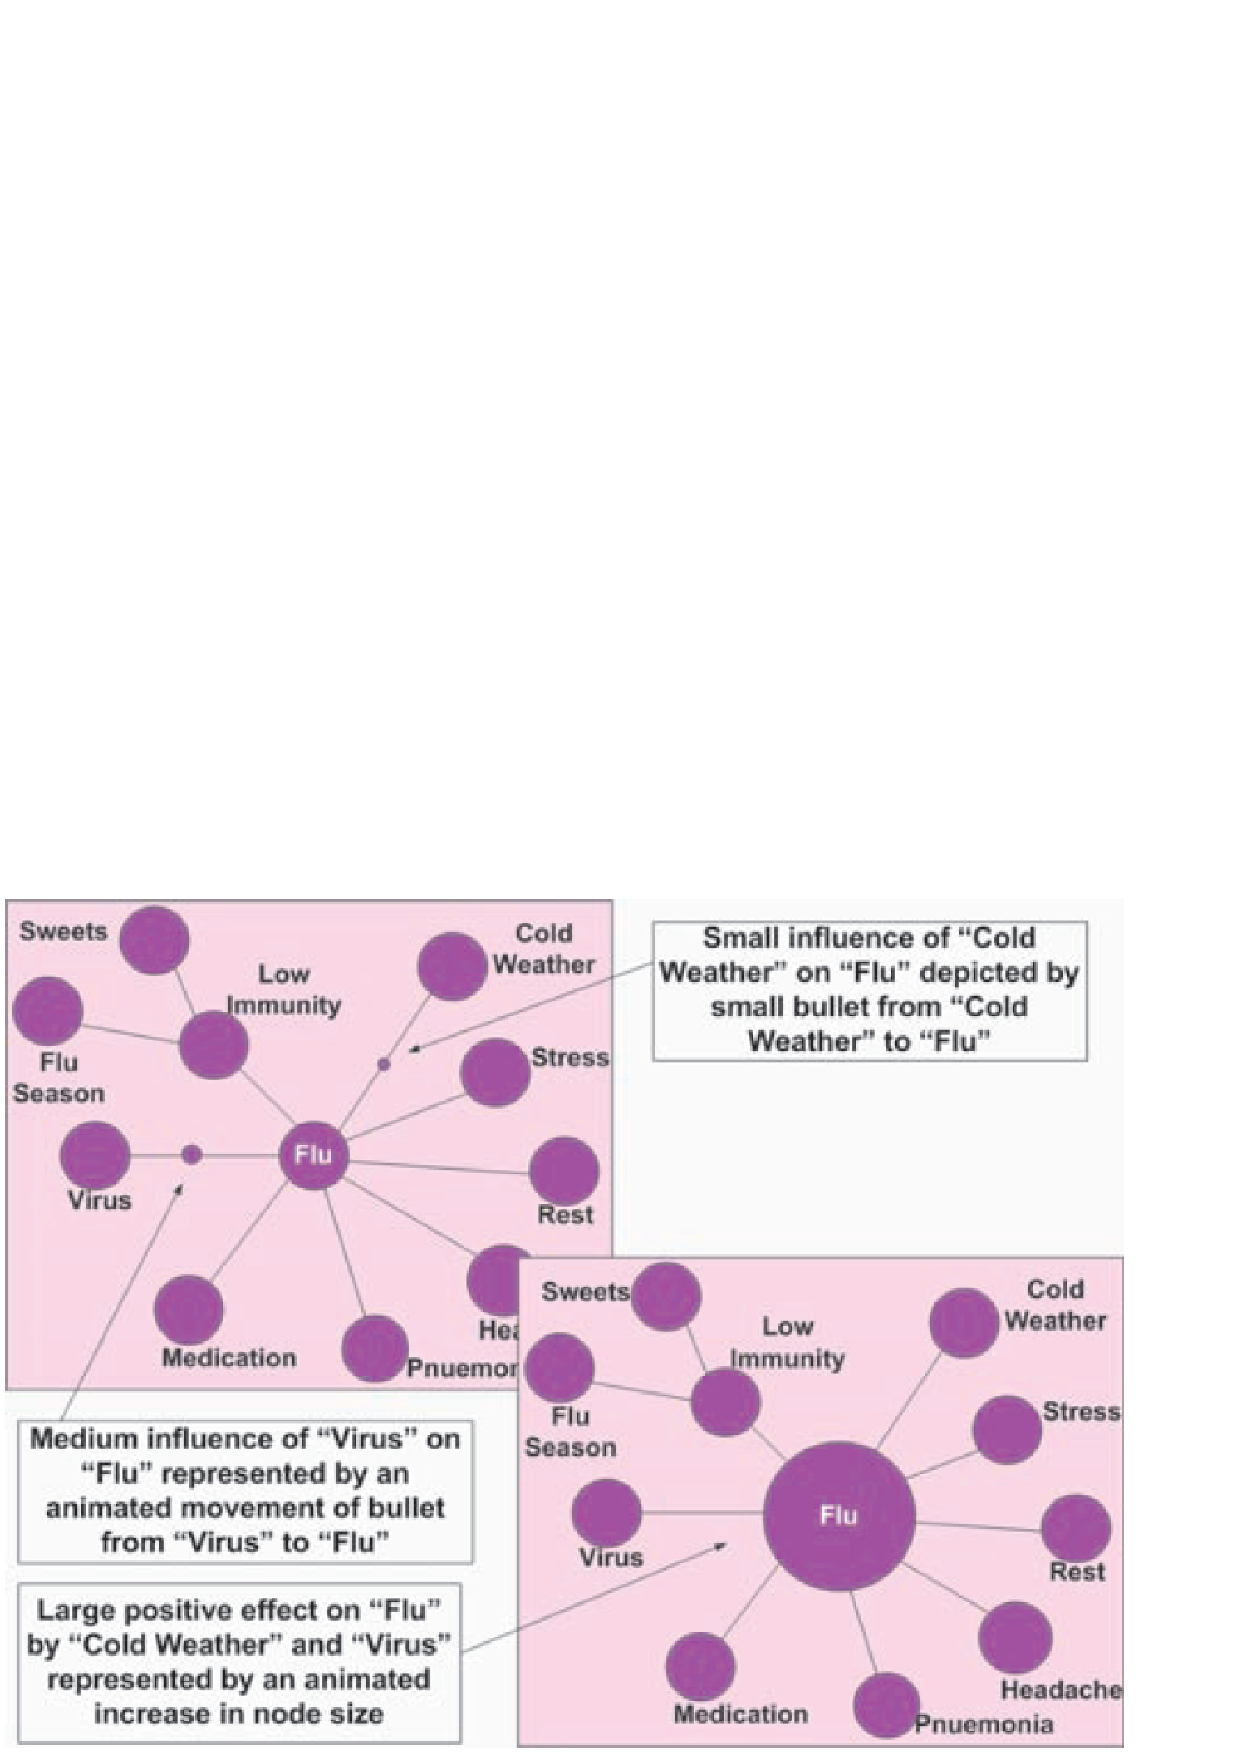
\includegraphics[width=0.46\textwidth]{figures/png/kadaba_animated.png}}

\caption[Two alternatives for visualizing causal influences]{Two alternatives for visualizing causal influences.  Reprinted from \textit{IEEE Transactions on Visualization and Computer Graphics}, Vol. 13, \citeauthor{kadaba2007}, Visualizing Causal Semantics using Animations, 1254--1261, \textcopyright \citeyear{kadaba2007}, with permission from IEEE.}

	\label{fig:kadaba}
\end{figure}

Kadaba et al.\ expanded upon Ware et al.'s VCV work to compare between static and animated causal visualizations \citeyearpar{kadaba2007}.  In their static design, positive influences were indicated with a plus sign ($+$) glyph and negative influences were indicated with a minus sign ($-$) glyph attached to the link between two entities in the network, as in Figure~\ref{fig:kadabaStatic}.  The size of the glyph represented the magnitude of the influence on the recipient node and glyphs of the same color described a multiplication effect on the recipient.   Their animated design featured bullets traveling along the links toward the recipient node to indicate causal influences, shown in Figure~\ref{fig:kadabaAnimated}.  As a bullet hit the recipient node, the size of the recipient node changed.  They found that subjects can interpret animated and static representations equally accurately, but subjects formed responses slightly quicker with animated representations.

\subsection{Uncertainty}

\begin{figure}
\centering

\subfigure[Error cone.]{\label{fig:uncertaintyCone}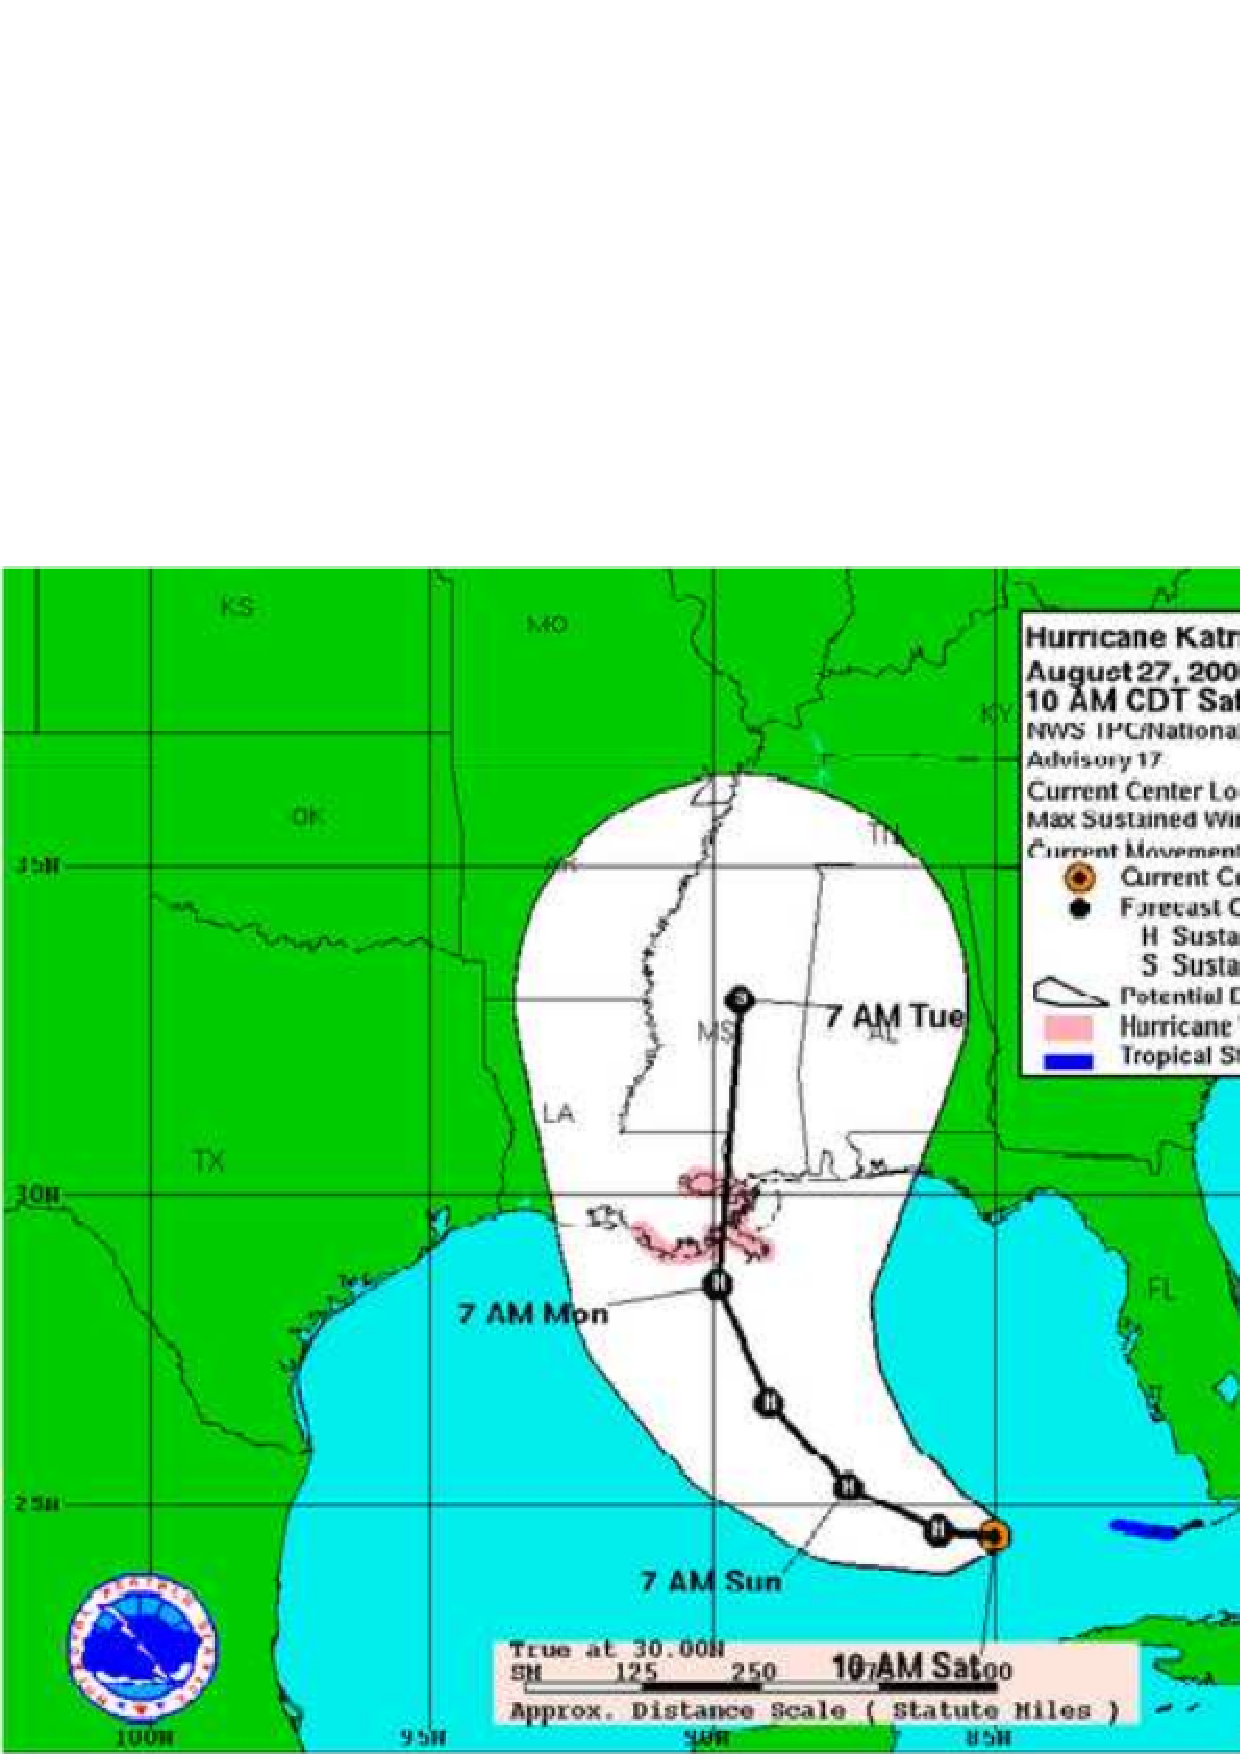
\includegraphics[height=4.5cm]{figures/png/uncertainty_cone.png}} 
\subfigure[Cox et al.'s method.]{\label{fig:uncertaintyHouse}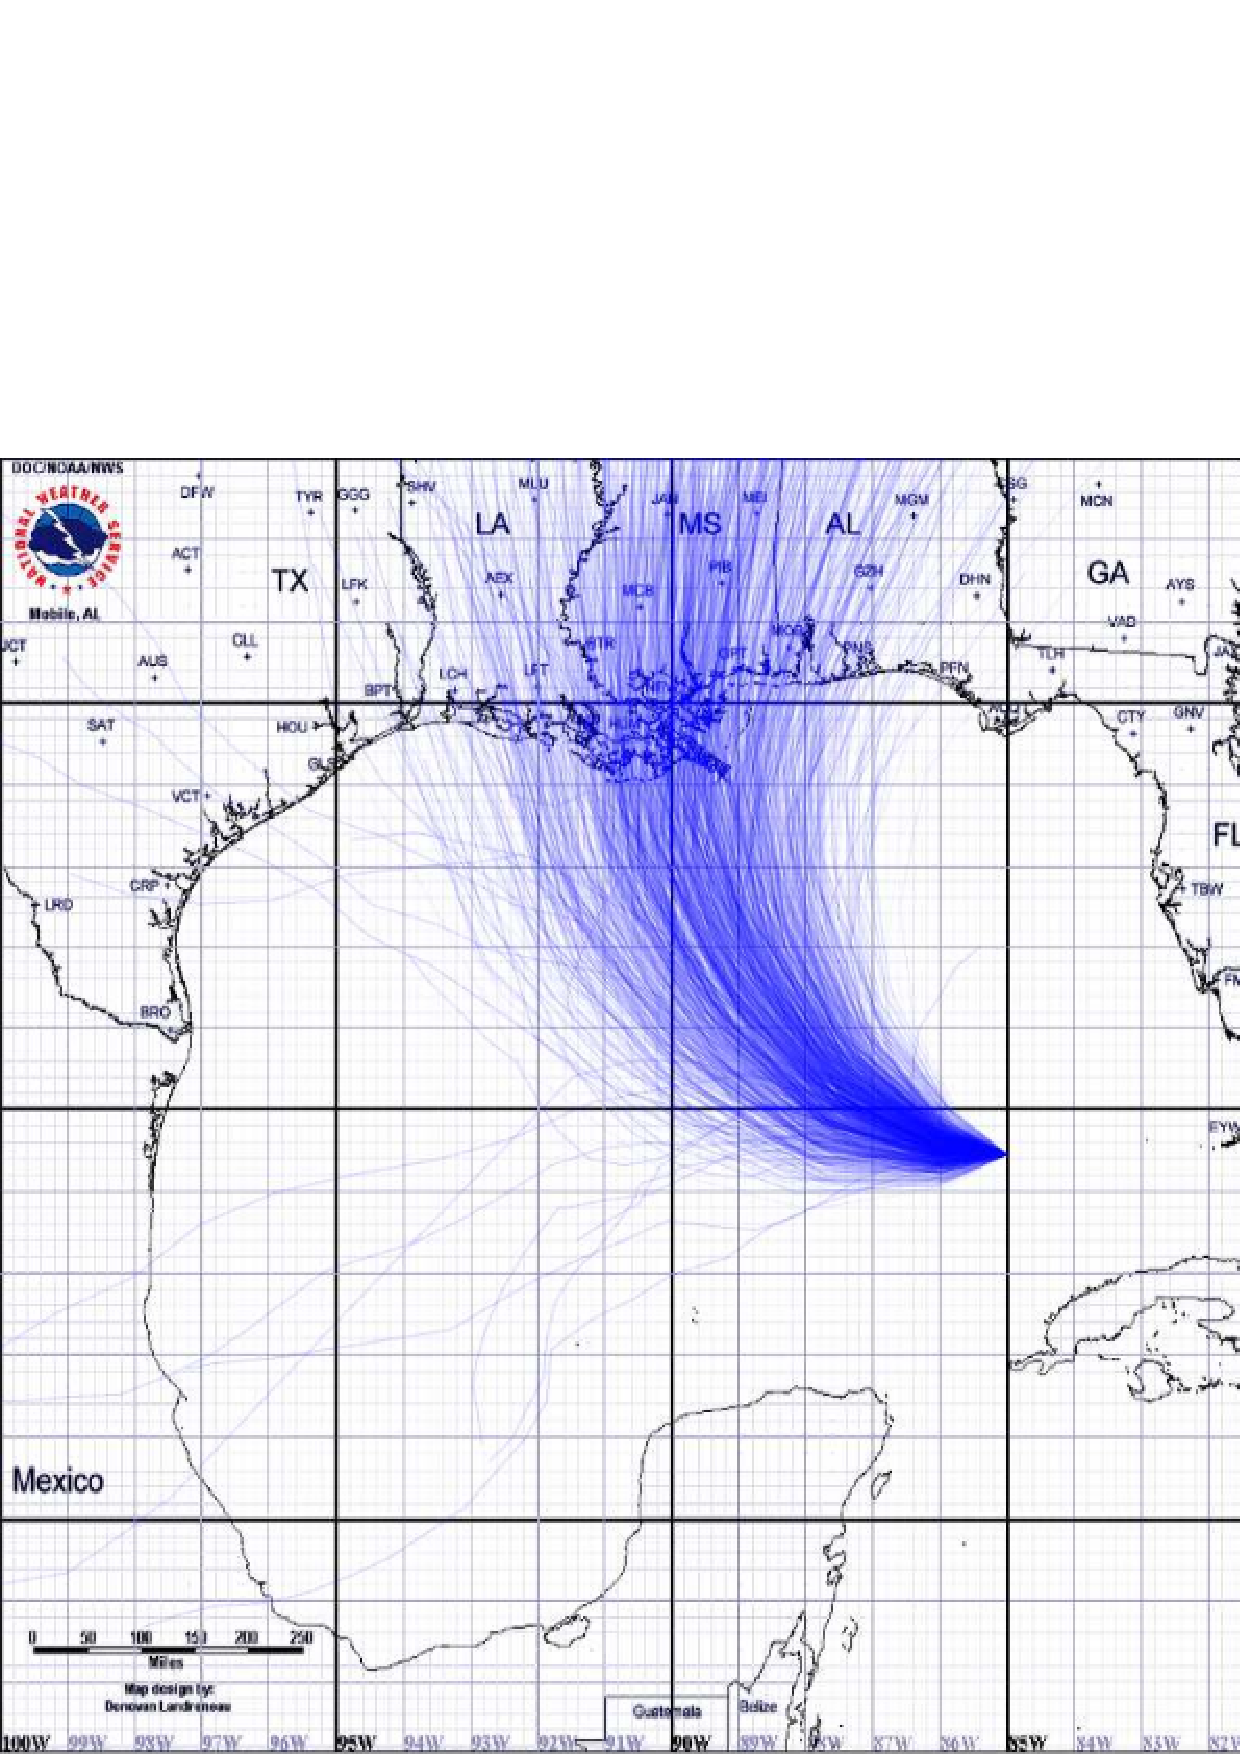
\includegraphics[height=4.5cm]{figures/png/uncertainty_house.png}}

\caption[Two visualizations of uncertainty for a hurricane advisory]{Two visualizations of uncertainty for a hurricane advisory.  Reprinted from \textit{International Journal for Uncertainty Quantification}, Vol. 3, \citeauthor{cox2013}, Visualizing Uncertainty in Predicted Hurricane Tracks, 143--156, \textcopyright \citeyear{cox2013}, with permission from Begell House, Inc.}

	\label{fig:uncertaintyAlternatives}
\end{figure}

Because a model is a simplification of reality, there are many reasons why it may be inaccurate.  There may be inaccurately estimated parameters used in the model, such as the predation matrix coefficients or the starting values for the biomasses of the fish species.  Furthermore, relevant factors may not have been taken into account when designing the model, such as climate.  Inaccuracies may even result from approximation techniques, such as the use of a Runge-Kutta method.  Therefore, it is common for a model's output to be regarded with some uncertainty.  To clarify, \textit{error} describes inaccuracies when the correct answer is known, while \textit{uncertainty} describes inaccuracies when the answer is unknown \cite{hunter1993}.  Due to uncertainty, model output is best understood as a range of expected values that is likely to contain the true value.  According to Potter et al., scientific data should be considered to be incomplete without representations of uncertainty \cite{potter2010}, so we have investigated some different portrayals of uncertainty.

Cox et al.\ explored methods for depicting uncertainty for hurricane advisories \citeyearpar{cox2013}.  The traditional error cone, shown in Figure~\ref{fig:uncertaintyCone}, is used by NOAA's National Hurricane Center, but it can be poorly understood by the average citizen.  Cox et al.\ designed their own alternative representation, shown in Figure~\ref{fig:uncertaintyHouse}, where many possible hurricane tracks are drawn to describe the range of possible outcomes.  Their user evaluation found that neither method was significantly better than the other for all cases, but a qualitative analysis showed that nearly all users prefer their new method over the error cone.

\section{Understanding Models}

Users studying models can benefit from the aid of a visualization, because patterns and trends may be difficult---if not impossible---to discern from only a table of numerical values.  The learning process can be even further enhanced through interaction with the model.  If interactivity is supported by the visualization, users can adjust parameter values, perceive a change (or perhaps no change) in the results, and begin to understand the degree of influence different parameters possess.

\subsection{Spreadsheet Programs}

\begin{figure}
\centering

\subfigure[A screenshot of VisiCalc.  GNU General Public License.]{\label{fig:visicalc}\includegraphics[height=4cm]{figures/png/visicalc.png}} \qquad
\subfigure[A chart made using Microsoft Excel.  Public domain.]{\label{fig:excel}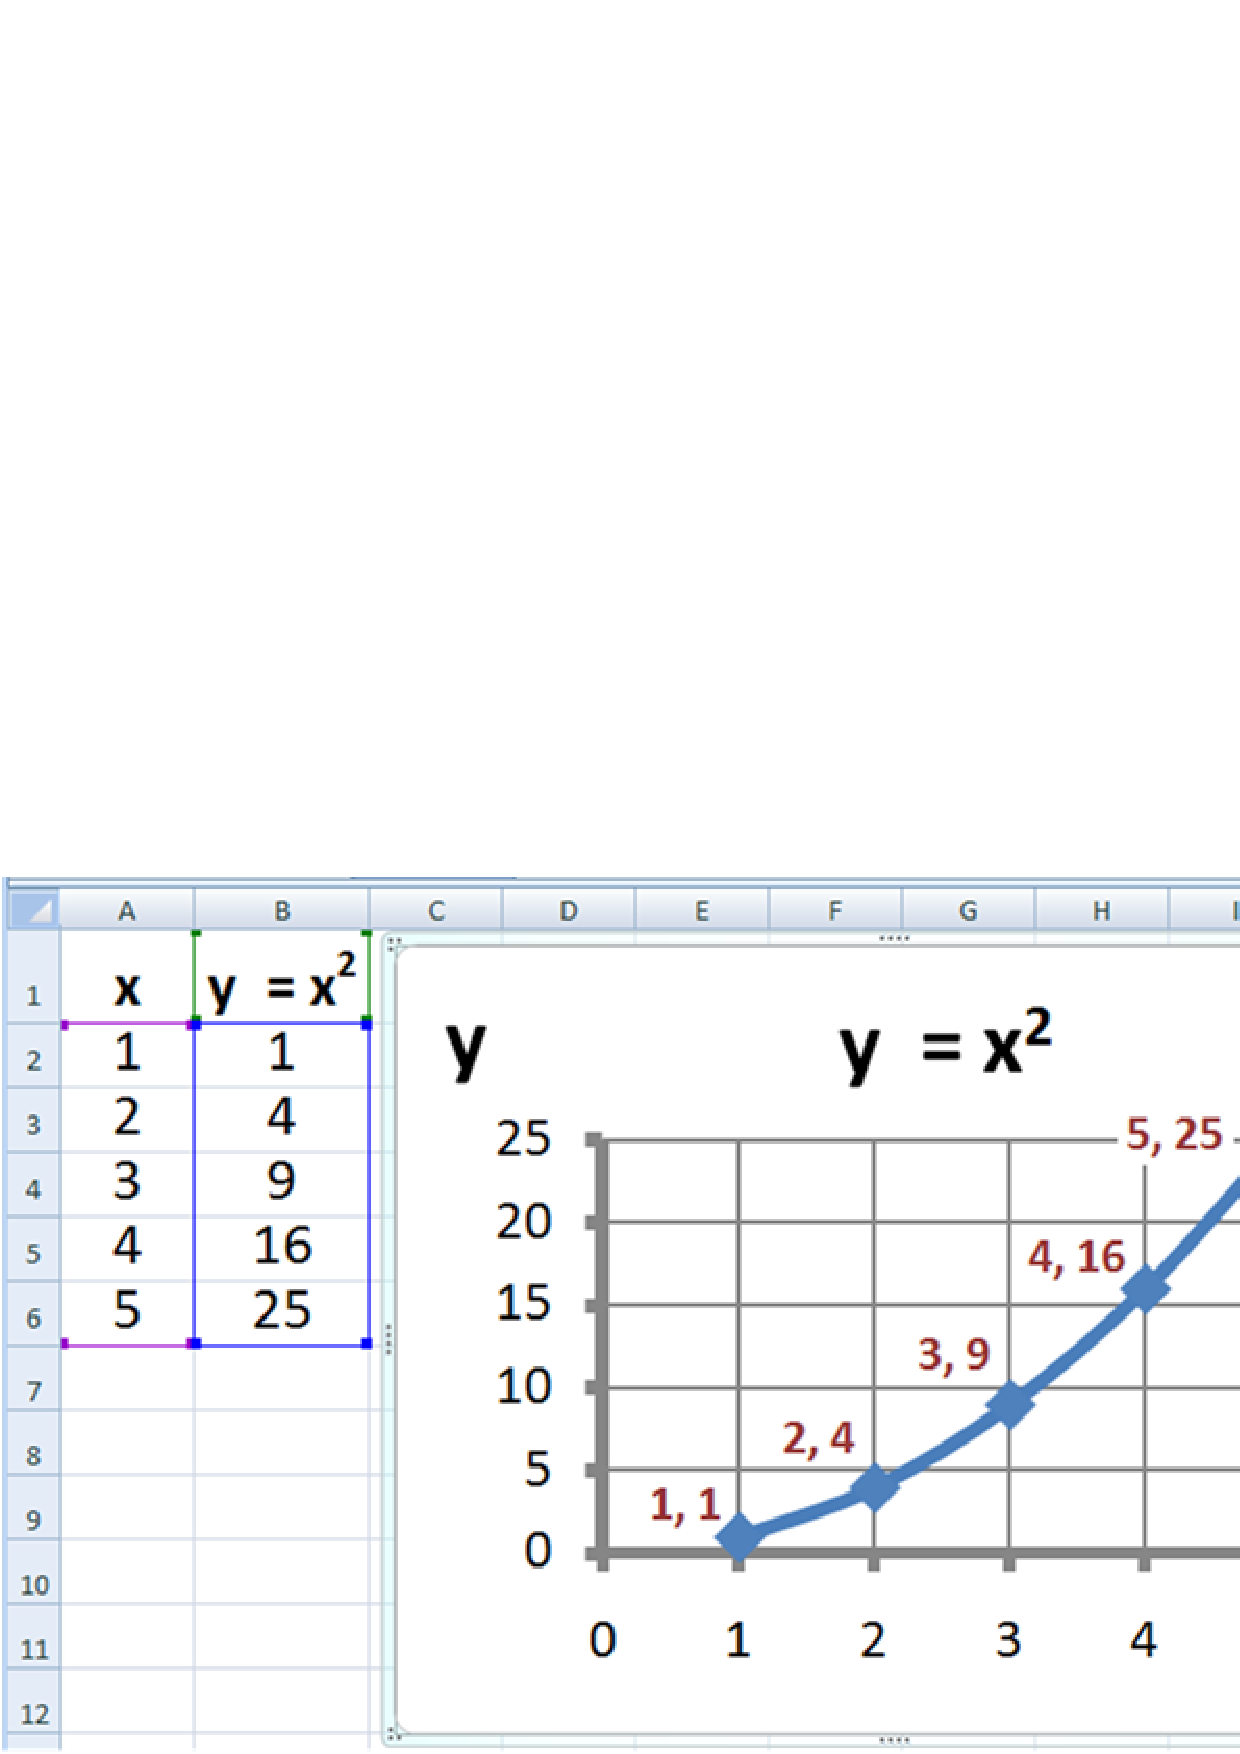
\includegraphics[height=4cm]{figures/png/excel.png}}

	\caption[Two examples of spreadsheet applications]{Two examples of spreadsheet applications.}
	\label{fig:spreadsheets}
\end{figure}

VisiCalc was a very early example of software assisting the understanding of models through visualizations \cite{grad2007}.  As a business student, Bricklin wished there was a faster way to change the input or fix mistakes when working out financial models by hand \citeyearpar{bricklin1999}.  To address this, he worked with Frankston to develop VisiCalc, seen in Figure~\ref{fig:visicalc}.  As the world's first electronic spreadsheet, VisiCalc consisted of rows and columns containing either text, numerical values, or formulas.  Result cells were instantly updated according to changed inputs or adjusted formulas, allowing a user to work with models in a more efficient and dynamic manner.  VisiCalc was superseded by Lotus 1-2-3, which was in turn supplanted by Microsoft Excel.  Microsoft Excel remains popular and features graphing tools that can generate charts, such as in Figure~\ref{fig:excel}.

\subsection{The Influence Explorer}

\begin{figure}[h]
	\centering
	\includegraphics[width=0.95\textwidth]{figures/png/influenceExplorer3.png}
	\caption[A screenshot of the Influence Explorer]{A screenshot of the Influence Explorer.  Image courtesy of Robert Spence.}
	\label{fig:influenceExplorer}
\end{figure}

The Influence Explorer by Tweedie et al.\ is a good example of a more complex interactive visualization \citeyearpar{tweedie1995}.  They developed an interface for understanding the relationships between different attributes in a design process.  Design parameter values of the Influence Explorer are initially randomly selected in a Monte Carlo simulation to represent many different possible designs.  Each cell in the histogram is a simulation run.  For each attribute, there is a histogram including each of the items.  The attribute ranges are controlled by sliders.  When the user adjusts the slider of a given attribute, all items that are within that range are highlighted on all of the histograms.  Figure~\ref{fig:influenceExplorer} is a screenshot of the Influence Explorer being used to test the performance of different light bulb designs; red indicates the design passed, while the black-to-white scale indicates the number of tests the design failed.  In a user evaluation, industrial designers found the ability to interactively explore the effects of different parameter ranges to be valuable.

\subsection{Vensim}

\begin{figure}[h]
	\centering
	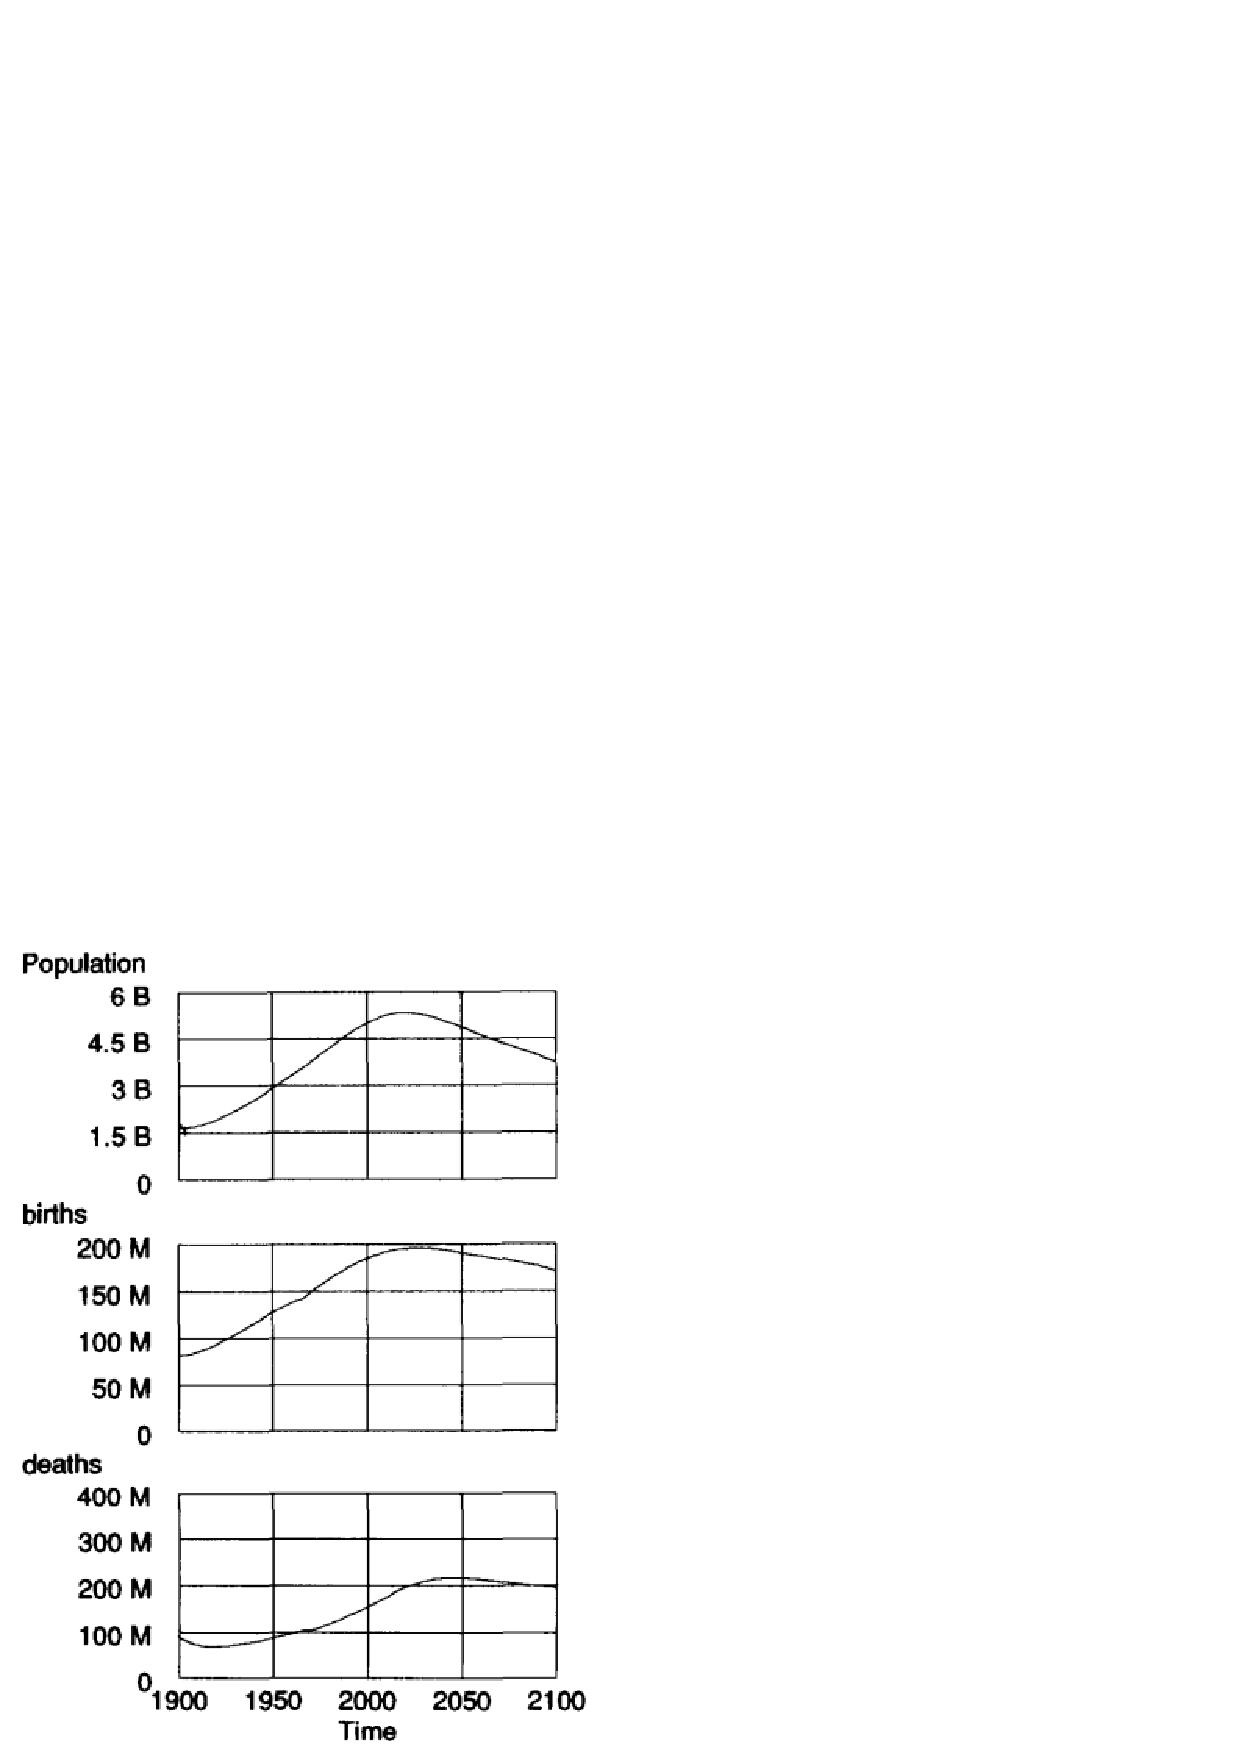
\includegraphics[width=6cm]{figures/png/vensim.png}
	\caption[A screenshot of the strip graphs in Vensim]{A screenshot of the strip graphs in Vensim.  Reprinted from \textit{European Journal of Operational Research}, Vol 59, \citeauthor{eberlein1992}, Understanding models with Vensim\texttrademark, 216--219, \textcopyright  \citeyear{eberlein1992}, with permission from Elsevier.}
	\label{fig:vensim}
\end{figure}

Eberlein and Peterson recognized that both unskilled and skilled model users have the same need: to quickly obtain a thorough understanding of a model and its implications \citeyearpar{eberlein1992}.  This motivated their development of Vensim, which is a commercial tool for visualizing and analyzing simulation results.  Vensim allows users to run a model under different conditions with a simple mouse click, enabling the user to learn the effects of different actions with ease.  Various features enhance this learning process---e.g., ``causal tracing'' strip graphs, shown in Figure~\ref{fig:vensim}.  Rather than simply seeing a chart of the projected population, a user exploring the causal tracing feature can begin to understand the various components that contributed to the population simulations---births and deaths---by seeing each component on its own chart.  A major emphasis of Eberlein and Peterson is that the same visualization tool can and should be used for both the development and teaching phases of a model, especially since those phases may not be discrete.
